\documentclass[11pt]{article}
% Shared preamble
\usepackage[papersize={8.5in,11in},textwidth=437pt,textheight=634pt,hcentering,top=81pt,headsep=22pt,headheight=16pt]{geometry}
\usepackage[T1]{fontenc}
\usepackage{lmodern}
\usepackage{mathtools,amssymb,amsthm}
\usepackage{microtype}
\usepackage{booktabs,array}
\usepackage[font=small,labelfont=bf,labelsep=period]{caption}
\usepackage[shortlabels]{enumitem}
\usepackage{needspace}
\usepackage{tikz}
\usetikzlibrary{calc,positioning,arrows.meta}
\definecolor{ink}{HTML}{213650}
\definecolor{sea}{HTML}{19706F}
\definecolor{rust}{HTML}{AA5034}
\usepackage[numbers,sort&compress]{natbib}
\renewcommand\bibfont{\small}
\usepackage[nottoc,notlof,notlot]{tocbibind}
\usepackage{fancyhdr}
\usepackage{url}
\usepackage[colorlinks,linkcolor=ink,citecolor=sea,urlcolor=ink,psdextra]{hyperref}
\usepackage{bookmark}

\fancyhf{}
\newcommand\shorttitle{OpenAI}
\fancyhead[L]{\small\scshape\shorttitle}
\fancyhead[R]{\small\thepage}
\renewcommand\headrulewidth{0pt}
\pagestyle{fancy}
\newcommand{\articletitle}[2]{\title{\fontsize{20}{24}\selectfont\bfseries\color{ink}#1}\renewcommand\shorttitle{#2}%
  \hypersetup{pdftitle={#1},pdfauthor={OpenAI}}}
\author{OpenAI}
\date{November 24, 2026}
\setcounter{tocdepth}{1}

\newtheorem{theorem}{Theorem}[section]
\newtheorem{lemma}[theorem]{Lemma}
\newtheorem{claim}[theorem]{Claim}
\newtheorem{corollary}[theorem]{Corollary}
\newtheorem{proposition}[theorem]{Proposition}
\theoremstyle{definition}
\newtheorem{definition}[theorem]{Definition}
\newtheorem{remark}[theorem]{Remark}
\newtheorem{example}[theorem]{Example}
\numberwithin{equation}{section}
\emergencystretch=1em
\clubpenalty=3500
\widowpenalty=3500
\raggedbottom

% For numbers of results in companion papers
\makeatletter
\newcommand\ext[2]{\@ifundefined{ref@#1:#2}{??\@latex@warning{Undefined companion label #1:#2}}{\csname ref@#1:#2\endcsname}}
\newcommand\extdef[3]{\@namedef{ref@#1:#2}{#3}}
\makeatother
\extdef{G}{lem:submod}{5.2}
\extdef{G}{prop:joint-convexity}{3.3}
\extdef{G}{sec:spectra}{2}
\extdef{G}{thm:main}{1.1}


\newcommand\titlebreak{\texorpdfstring{\\}{}}
\settocbibname{References}

% Lightweight contents, with numbered bookmarks
\bookmarksetup{numbered}
\makeatletter
\renewcommand\@pnumwidth{2.1em}
\renewcommand\@dotsep{12}
\renewcommand*\l@section[2]{\addvspace{.45em}\@dottedtocline{1}{\z@}{2em}{#1\nobreak\hspace{.5em}}{#2}}
\makeatother

\articletitle{The logarithmic exponent \titlebreak of finite Fourier transforms}{The logarithmic exponent of finite Fourier transforms}
\hypersetup{pdfsubject={The-logarithmic-exponent-of-finite-Fourier-transforms-November-24-2026}}
\usetikzlibrary{fit,backgrounds,decorations.pathreplacing,matrix}
\newcommand{\Q}{\mathbb Q}
\newcommand{\Z}{\mathbb Z}

\begin{document}
\maketitle

\begin{abstract}
The minimum number of binary linear gates for a finite abelian Fourier
transform of order $N$ is $N(\log N)^{1/2+o(1)}$. This holds over every
field in which $N$ is invertible and which contains the required roots
of unity. The same cost per transform holds for any number of independent
inputs, even when gates can mix them. Formal polynomial multiplication
has the same logarithmic exponent over every field, including for
batches of independent products.
\end{abstract}

\section{Introduction}\label{sec:intro}

Each coefficient of a discrete Fourier transform is a weighted sum of
all the input samples. Computing the sums separately takes quadratic
work. The fast Fourier transform shares partial sums among frequencies
and, at power-of-two lengths, computes all $N$ outputs in
$O(N\log N)$ operations \cite{CooleyTukey}. How much of that
logarithmic work per sample is intrinsic? A linear circuit may choose
arbitrary scalar coefficients and reuse any intermediate result.

We prove that the optimal logarithmic exponent is $1/2$. A circuit
needs at least order $\sqrt{\log N}$ gates per sample, and for every
$\epsilon>0$ we construct circuits using
$O_\epsilon((\log N)^{1/2+\epsilon})$ gates per sample. The bounds hold for every finite abelian group whose order is
invertible in the field and whose characters take values there. They
also hold per sample when one circuit processes many independent
signals, even if its gates combine values from different signals.

Write $C_K(T)$ for the smallest number of gates in an acyclic linear
circuit computing a matrix $T$ over a field $K$. Each gate forms
$au+bv$ from two available values, with arbitrary $a,b\in K$. An
output may select and scale a single input or gate value, or return
zero. All logarithms in the paper are to base two.

\begin{theorem}[The Fourier exponent]\label{thm:main}
Let $G_1,\ldots,G_J$ be finite abelian groups of common order $N\ge2$,
where $J\ge1$. Suppose $N$ is invertible in $K$ and $K$ contains a
primitive root of unity of order $\exp(G_j)$ for each $j$. Let $T$ be
the direct sum of their Fourier transforms, choosing the forward or
inverse transform independently in each block. For an absolute $c>0$
and a constant $C_\epsilon$ depending only on $\epsilon>0$,
\[
 c\,JN\sqrt{\log N}\ \le\ C_K(T)\
            \le\ C_\epsilon\,JN(1+\log N)^{1/2+\epsilon}.
\]
\end{theorem}

\needspace{4\baselineskip}
Here $\exp(G)$ is the exponent of the group. The field condition gives
one frequency for each character $\chi:G\to K^\times$. The forward
transform sends a list $(x_g)_{g\in G}$ to the list of sums
$\sum_{g\in G}\chi(g)x_g$, one for each $\chi$. For example, on
$(\mathbb Z/2\mathbb Z)^k$ over $\mathbb C$ these are the
Walsh--Hadamard sums, with coefficients $+1$ and $-1$. Each of $J$
independent Walsh--Hadamard transforms of length $2^k$ costs at least
$c\,2^k\sqrt{k}$ gates on average, however fast $J$ grows with $k$.
Theorem~\ref{thm:main} leaves open an upper bound with $\epsilon=0$.

The exponent also governs \emph{formal polynomial convolution}, the
map that takes two lists of $n$ coefficients to the coefficients of
their polynomial product. Over every field, $J$ independent products
require $\Omega(Jn\sqrt{\log n})$ gates in a division-free arithmetic
circuit, and $O_\epsilon(Jn(1+\log n)^{1/2+\epsilon})$ gates suffice
(Corollary~\ref{cor:conv-exponent}). Here addition, subtraction and
multiplication are binary operations, including multiplication by a
prescribed scalar. For the Fourier transform itself, allowing products
of intermediate polynomials in an exact formal circuit also gives the
same exponent. Taking the linear part of each gate turns a product
$uv$ into $u_0v_1+v_0u_1$, where the subscripts denote constant and
linear parts. Conversely, three field operations suffice for a weighted
linear gate.

\subsection{A lower bound with feedback and errors}

The lower bound allows two further ways in which a circuit might save
work. First, it may use feedback. A system of $s$ scalar states
specifies each state as a weighted sum of at most two inputs or
states, with a unique solution for every input. Write $\mathcal C_s(h)$
for the $h$-input, $h$-output matrices computed in this way over
$\overline K$ using at most $s$ states and the readout convention
above. Second, the system may leave behind a low-rank error and an
error concentrated on a prescribed number of matrix entries. Each
can couple all the blocks. Even a limit of these corrected systems
obeys the lower bound.

\begin{theorem}[Robust lower bound]\label{bch:uniform-robust}
With $T$ as in Theorem~\ref{thm:main} and $h=JN$, there are absolute
constants $c,\beta,\eta>0$ with the following property. Suppose $T$
belongs to the Zariski closure over $\overline K$ of all sums $M+B+Z$
satisfying
\[
 M\in\mathcal C_s(h),\qquad \operatorname{rank}B\le\beta h,\qquad
 |\operatorname{supp} Z|\le\eta h\,2^{\sqrt{\log N}/8}.
\]
Then $s\ge c\,h\sqrt{\log N}$.
\end{theorem}

The support budget counts nonzero entries in the entire $h\times h$
matrix. Taking the closure of the sums lets the feedback matrix and
both corrections vary together. Setting the corrections to zero and
using an acyclic circuit gives the lower bound of Theorem~\ref{thm:main}.

\subsection{Earlier bounds for Fourier circuits}

The classical $O(N\log N)$ count has two ingredients. Cooley and
Tukey factor a transform of length $ab$ into transforms along the two
axes, with a diagonal scaling between them. Good's factorization
eliminates the scaling for coprime lengths
\cite{Good,CooleyTukey,cooleyLewisWelch1967}. Recursing on powers of
two gives the familiar FFT. Bluestein's reduction to convolution
with a fixed quadratic phase, followed by padding to a power of two,
gives the same asymptotic count for every complex transform length
\cite{Bluestein,rabinerSchaferRader1969}.

Several classical lower bounds explain when this count is necessary.
Papadimitriou proved optimality under restrictions on the paths in
the computation graph \cite{Papadimitriou}. Winograd counted multiplications
separately from additions \cite{Winograd1979DFT}. For the unnormalized
complex transform, the determinant has modulus $N^{N/2}$.
Morgenstern showed that if scalar multipliers have modulus at most one,
an addition can at most double the largest determinant modulus
attainable from the available forms. At least $\tfrac12N\log_2 N$
additions are therefore necessary \cite{Morgenstern}. Normalizing the
transform makes its determinant have modulus one. For this transform,
Ailon proved an $\Omega(N\log N)$ lower bound for in-place
two-coordinate unitary operations, and an $\Omega(N\log N/R)$ bound
for in-place rotations and scalings when every intermediate map has
condition number at most $R$ \cite{Ailon,AilonCondition}.
Theorem~\ref{thm:main} permits arbitrary scalar coefficients,
intermediate storage and reuse.

For power-of-two lengths, Alman and Rao used matrix nonrigidity to
reduce the leading operation counts to $\tfrac{23}{24}N\log_2 N$
for Walsh--Hadamard transforms over a field and $\tfrac{15}{4}N\log_2 N$
in real arithmetic for complex cyclic transforms, up to $O(N)$ terms
\cite{AlmanRao}. Finite tensor constructions subsequently gave
$o(N\log N)$ circuits along a subsequence \cite{FiniteFourier}.
At every length, the algorithm of \cite[Theorem~1.1]{ExplicitFourier}
uses a finite network from \cite[Proposition~8 and Section~3.5]{Tape}
to save a fixed positive power of $\log N$. It charges for array indexing and for preparing the
scalars from a supplied root of unity of polynomial order.
Sussman developed a recursion that handles several target maps
together \cite{Sussman}. Kartal combined it with constructions of
CubeJerry, Cinna Davis and Ali Romman, and Yao and Liu refined the
resulting numerical bounds \cite{Kartal,kartalpi,YaoLiu}. A subsequent
construction gives a saving greater than $0.0039$ in this complex
arithmetic model \cite{RelayFourier}. The circuit size in Theorem~\ref{thm:main}
charges only for the binary linear gates.

Valiant related linear circuits to matrix rigidity, the number of
entries that must change to reach a prescribed rank
\cite{Valiant1975,Valiant1977}. Alman and Williams showed that the
Walsh matrix fails Valiant's rigidity criterion \cite{AlmanWilliamsRigidity}.
For every fixed $\delta>0$, Dvir and Liu reduce the rank of any
sufficiently large complex abelian character table to
$o(N/\log\log N)$ by changing at most $N^{1+\delta}$ entries
\cite[Theorem~6.1]{DvirLiu}. Theorem~\ref{bch:uniform-robust},
with one transform and no circuit states, gives a lower bound in the
same variables. Reducing the rank to $\beta N$ requires more than
$\eta N2^{\sqrt{\log N}/8}$ changes. For a smaller target rank, Alman
showed that reducing a Walsh matrix over $\mathbb F_3$ to rank
$\lfloor(\log_2 N)^2/80\rfloor$ requires changing more than one percent
of its entries \cite{AlmanRigidity}.

For convolution, specializing one input turns a bilinear circuit into
a linear one. Raz used specialization for bounded-coefficient matrix
multiplication \cite{Raz}. B\"urgisser and Lotz proved an
$\Omega(n\log n)$ bound for complex cyclic convolution and ordinary
polynomial multiplication in the bounded-coefficient bilinear model
\cite{BurgisserLotz}.
Corollary~\ref{cor:conv-exponent} uses a fixed operand over the algebraic
closure to obtain a Fourier transform, giving a lower bound for
division-free formal polynomial multiplication with arbitrary scalars
over every field.


\subsection{Where the square root enters}

\paragraph{A geometric test for a small circuit.}
Rank and the number of nonzero entries each describe one way a matrix
can be easy to compute. Neither by itself explains the Fourier bound.
For example, over $\mathbb Q$ the map that adds the sum of all inputs
to each input is dense and invertible, yet has a linear-size circuit.
Part~\ref{part:lower} tests rank and support together by placing the
indices of a matrix at the corners of a rectangle. The construction
uses the tensor prices of the companion geometry paper \cite{oaG}.
A wire sharing one of $q$ labels between two sites costs their
distance times $\log q$. Placing the row label at both left corners
and the column label at both right corners gives a price that reads
log rank when the rectangle has height zero and log support size when
it has width zero, per unit of the remaining length.

At width one and height $L$ the price of a character table is exactly
$(L+\sqrt{1+L^2})\log N$ (Theorem~\ref{geo:saturation}). A
permutation matrix at the same placement costs $(L+1)\log N$. Both
matrices have full rank. As the rectangle opens up, their prices
separate by approximately $\tfrac12 L^2\log N$. Thus even at height
of order $1/\sqrt{\log N}$ the test detects a difference of constant
size. To obtain the exact Fourier price, we use two diagonal
character phases and changes of basis to exchange the two labels.
The cost of this exchange forces the character table to attain the
upper bound from supplying its labels through the center.

The circuit comparison applies the rectangle test to the list of both
inputs and outputs of a transform. Pairing two copies of the list
exposes the character table, and the resulting lower bound on the
list survives a small fractional loss of rank. For a batch, eliminating
a single rank correction that mixes the signals might seem to destroy
every individual list. Row reduction and a scaling limit recover a
separate projection on each block. Their rank losses add up to at
most the original rank budget, so most blocks retain the lower bound.

Finally, repeat each scalar input and state along $d$ time coordinates.
A shift at every state leaves a copy of the desired transfer on each
time diagonal. Changing the shift by a map of rank one kills every
path that runs through $d$ states. The short paths left behind reach
at most $2^{d-1}$ inputs per output, while the total rank correction
costs at most one dimension per state. With $d$ of order
$\sqrt{\log N}$, the list test rules out the resulting combination
of rank and support unless the circuit has at least a constant times $JN\sqrt{\log N}$
states (Section~\ref{bch:proof:section}).

\paragraph{Predicting a product and repairing it exactly.}
The upper bound in Part~\ref{part:finite} starts with the Walsh--Hadamard
transform. We express a transform on many binary digits, up to
permutations and scalings, as a product of $m$ commuting operators.
In their common frequency basis each operator multiplies by a sign.
The product is determined by the parity of the number of negative
signs. Run many independent inputs together and assign them all
possible sign shifts in equal proportions. At each frequency the
shifted count has a binomial distribution over the batch. Almost all
counts lie in an interval of width $O(\sqrt{m\log m})$, on which a
polynomial of that degree gives the parity sign exactly. Undoing the
known shift gives the desired answer on those rows.

The exceptional rows depend on the frequency. Converting every input
to the common basis to correct them would spend the work we are trying
to save. Instead, send a small number of linear combinations of the
rows into the frequency basis. There the exceptional positions are
known, and interpolation recovers the corrections from those combinations.
A fixed number of further predictor applications in ordinary
coordinates then corrects every output (Theorem~\ref{thm:repair}).

A degree bound for the predictor still has to become a gate bound.
We evaluate it in $O(\sqrt{m\log m})$ stages, each a matrix linear
in the commuting operators. A stage may ask for short Fourier
transforms in $m$ different directions. The construction in
Section~\ref{sec:prime-kernel} shares those calls among rows by
factoring their routes through common source and destination maps.
It uses different characteristics for the routing labels and the
addresses, drawing on constructions in \cite{Tape,FranklWilson1981,Alon1998}
and related ideas in index coding \cite{BarYossefBirkJayramKol2006,LubetzkyStav2009}.
For any fixed $\theta>1/2$, a finite choice of parameters then
replaces a transform on $Af$ digits by fewer than $A^\theta$
transforms on $f$-digit axes per input row, averaged over the batch.
A single large transform already contains the independent inputs this
step needs. Holding some digits fixed gives disjoint slices on which
the remaining digits are transformed, and these slices fill the batches
in the recursion. Iterating gives the exponent on prime tensor powers.
In the binary
case the construction also controls how errors in individual gates
affect the normalized transform (Proposition~\ref{prop:binary-template}).
The tape multiplication paper uses this implementation \cite{oaT}.

\paragraph{Returning to the given field.}
A general finite abelian group factors into cyclic groups of different
orders. Even when the field contains every character of the original
group, a fast algorithm may call for roots of unity at other lengths.
Part~\ref{part:all} packs independent data into the coordinates of
small field extensions and charges the operations there back to the
base field. For formal convolution in characteristic zero, a single
deformation parameter handles all cyclic factors at once. In positive
characteristic, finite-field extensions supply roots with short
Frobenius periods. The resulting multiplication circuits over the
original field give fast evaluation and interpolation on geometric
grids, of which every cyclic Fourier matrix is an instance
(Theorems~\ref{thm:conv} and~\ref{up:grid}).
In the reverse direction, fixing one operand of a polynomial product
realizes a cyclic Fourier transform after diagonal scalings. Applying
the Fourier lower bound to this specialization gives the convolution
lower bound in Corollary~\ref{cor:conv-exponent}.

\medskip
{\small\tableofcontents}
\clearpage

\part{A joint test of rank and support}\label{part:lower}
\section{The spectral price of a character table}\label{geo:section}

The lower bound needs a test that sees rank and sparsity at the same
time. To build it, give a matrix two copies of its row index and two
copies of its column index. For a nonzero $N$-by-$N$ matrix $M$ over
the algebraic closure $k$ of the coefficient field, this is the tensor
of the diagonal operator
\[
    C_M(e_x\otimes e_y)=M_{xy}\,e_x\otimes e_y .
\]
Put the input legs at $A,B$ and the output legs at $A',B'$. Bringing
$A$ to $A'$ and $B$ to $B'$ exposes $M$ across the two remaining sites.
Bringing $A$ to $B$ and $A'$ to $B'$ exposes a diagonal matrix with the
entries of $M$ on its diagonal. The two resulting ranks are
$\operatorname{rank}M$ and $|\operatorname{supp}M|$.
Between these placements, the planar price from the companion paper
\cite{oaG} gives a continuous test of the same four-legged tensor.
A character table attains the largest possible price at every rectangle
(Theorem~\ref{geo:saturation}).

\subsection{Prices of placed tensors}

A price gives a lower bound on the cost of supplying a tensor by
wires between sites, allowing linear operations at each site. A
\emph{restriction} is one such operation applied at every site, after
grouping all indices there. On a fixed set of sites, tensor products
group the corresponding factors and direct sums separate the summands
at every site. In Strassen's asymptotic spectrum a \emph{spectral
point} is a restriction-monotone semiring homomorphism from these
tensors to $\mathbb R_{\ge0}$ that preserves zero and one
\cite{StrassenSpectrum}. We use logarithms to base two.

\begin{theorem}[Spectral plane and copying]\label{geo:spectrum}
Over an algebraically closed field $k$ of any characteristic there is an
assignment of a real price $H(T;\mathbf x)$ to each nonzero tensor $T$
with legs at any finite list of positions $\mathbf x$ in the Euclidean
plane. This assignment has the following properties.
\begin{enumerate}
\item A tensor at one site costs zero. For a finite set $S$ of positive
diameter we have $H(T;\mathbf x)=\delta(S)\log\Phi_S(T)$, where $\Phi_S$ is a
spectral point and $\delta(S)$ is half the perimeter of the convex hull
of $S$. For a segment its perimeter is twice its length. The prices
$H$ agree upon insertion of trivial legs.
\item A common label of $q$ values on all sites of a nonempty $S$, represented by
the diagonal tensor $\sum_{a=1}^q\bigotimes_{x\in S}e_a$, costs
$\delta(S)\log q$. In particular a wire of dimension $q$ between $X,Y$
costs $|X-Y|\log q$. Contracting tensor indices placed at a common
site is a local linear map.
\item The price of a fixed tensor is jointly convex and positively
homogeneous in its positions and invariant under simultaneous
translation. At a fixed placement, its sublevel sets, with the zero
tensor adjoined, are Zariski closed in every finite tensor format.
\item Suppose a basis label of width $q$ has the same value on legs at
$X$ and $Y$ throughout the support of $T$. An additional copy of that
label at $Z$ increases the price by at most
\begin{equation}\label{geo:copy}
 \tfrac12\bigl(|X-Z|+|Y-Z|-|X-Y|\bigr)\log q.
\end{equation}
\end{enumerate}
\end{theorem}

For the construction and the copying inequality, see \cite[Theorem~\ext{G}{thm:main}, Section~\ext{G}{sec:spectra} and Propositions~\ext{G}{prop:joint-convexity} and~\ext{G}{lem:submod}]{oaG}. The closedness of spectral sublevels is also proved in \cite{SpectralSublevels}. 
If several pairs of matching labels join
segments through $O$, we may copy all these labels to $O$ at zero
cost. A linear functional there multiplies the coefficients by any
prescribed function of the labels. When the multiplier is nonzero on
the support, the reciprocal gives price equality.

We write $P_M(A,B,A',B')=H(C_M;A,B,A',B')$ for $M\ne0$. To move
a leg, introduce a wire of the same dimension and contract one end
against the leg. The wire price bounds the cost of the move.
For a tensor $T$ put $h_T(\mathbf x)=H(T;\mathbf x)$.
Joint convexity and homogeneity give subadditivity in the positions.
For sums of tensors at a single fixed placement, the appropriate
subadditivity is instead
\begin{equation}\label{geo:sum}
   \Phi_S\Bigl(\sum_j T_j\Bigr)\le\sum_j\Phi_S(T_j).
\end{equation}
Indeed an ordinary sum is a restriction of the direct sum.
Multiplicativity of the spectral point makes the price of a grouped product the sum of the prices of its factors.

\subsection{The rectangle test}

Put the row label $x$ on the left side of a rectangle of height $L$ and
width $W$ and the column label $y$ on the right. The top corners
are $A=(-W/2,L/2)$ and $B=(W/2,L/2)$, with $A',B'$ directly below.
Write $P_M(L,W)$ for the price of this placement, $m=\log N$ and
$D=\sqrt{L^2+W^2}$ for its diagonal length.

Between two sites, row and column operations turn a tensor of flattening
rank $r$ into a wire of dimension $r$. Collapsing a side of the
rectangle therefore gives the rank and support readings
\begin{equation}\label{geo:endpoints}
   P_M(0,W)=W\log\operatorname{rank}M,\qquad
   P_M(L,0)=L\log|\operatorname{supp}M|.
\end{equation}
At the full rectangle the two different labels may both be copied
to its center $O$, as in Figure~\ref{geo:rectangle-figure}.

\begin{figure}[!htbp]
\centering
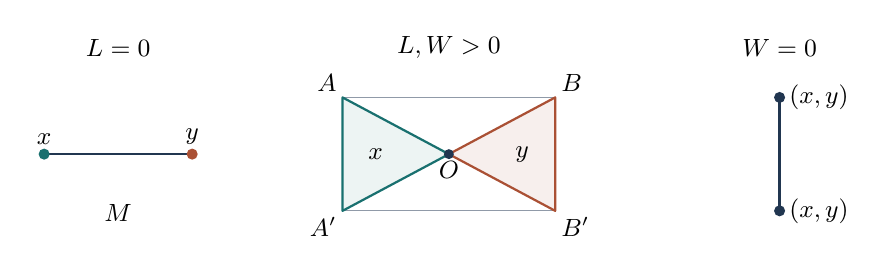
\begin{tikzpicture}[font=\small,line cap=round,line join=round]
 \begin{scope}[xshift=-4.2cm]
  \node at (0,1.35) {$L=0$};
  \draw[thick,ink] (-.94,0)--(.94,0);
  \fill[sea] (-.94,0) circle (2pt);
  \fill[rust] (.94,0) circle (2pt);
  \node[above] at (-.94,0) {$x$};
  \node[above] at (.94,0) {$y$};
  \node at (0,-.75) {$M$};
 \end{scope}
 \begin{scope}
  \node at (0,1.35) {$L,W>0$};
  \fill[sea!8] (-1.35,.72)--(-1.35,-.72)--(0,0)--cycle;
  \fill[rust!9] (1.35,.72)--(1.35,-.72)--(0,0)--cycle;
  \draw[ink!50] (-1.35,.72)--(1.35,.72) (-1.35,-.72)--(1.35,-.72);
  \draw[thick,sea] (-1.35,.72)--(-1.35,-.72)--(0,0)--cycle;
  \draw[thick,rust] (1.35,.72)--(1.35,-.72)--(0,0)--cycle;
  \node[above left,inner sep=2pt] at (-1.35,.72) {$A$};
  \node[below left,inner sep=2pt] at (-1.35,-.72) {$A'$};
  \node[above right,inner sep=2pt] at (1.35,.72) {$B$};
  \node[below right,inner sep=2pt] at (1.35,-.72) {$B'$};
  \node at (-.93,0) {$x$};
  \node at (.93,0) {$y$};
  \fill[ink] (0,0) circle (1.8pt);
  \node[below,inner sep=2.5pt] at (0,0) {$O$};
 \end{scope}
 \begin{scope}[xshift=4.2cm]
  \node at (0,1.35) {$W=0$};
  \draw[thick,ink] (0,-.72)--(0,.72);
  \fill[ink] (0,.72) circle (2pt) (0,-.72) circle (2pt);
  \node[right] at (0,.72) {$(x,y)$};
  \node[right] at (0,-.72) {$(x,y)$};
 \end{scope}
\end{tikzpicture}
\caption{At height zero the two-site matrix is $M$ in its row and
column labels. At width zero it is diagonal in the pair $(x,y)$.
In the middle, a common row label and a common column label supply the
two shaded triangles. Each triangle has semiperimeter $(L+D)/2$, and
a functional at $O$ multiplies their coefficient by $M_{xy}$.}
\label{geo:rectangle-figure}
\end{figure}

Sharing $x$ among $A,A',O$ and $y$ among $B,B',O$ costs the sum of
the two triangle prices. The local functional
$e_x\otimes e_y\mapsto M_{xy}$ at $O$ supplies the entry for free.
Consequently
\begin{equation}\label{geo:upper}
          P_M(L,W)\le (L+D)m
\end{equation}
even when some of the sites coincide.

\begin{theorem}[Price on a rectangle]\label{geo:saturation}
Let $N\ge1$ and $L,W\ge0$. Every nonzero $N$-by-$N$ matrix over $k$
has rectangle price at most $(L+\sqrt{L^2+W^2})\log N$. For the full
character table $F_G$ of any finite abelian group of order $N$
invertible in $k$,
\[
       P_{F_G}(L,W)=(L+\sqrt{L^2+W^2})\log N .
\]
More generally the supremum of the rectangle prices in any family
satisfying Proposition~\ref{geo:first-phase} equals this upper bound.
\end{theorem}

A permutation matrix, by comparison, uses one common label of size $N$
on the four corners. After relabeling the legs its tensor is precisely
that diagonal, of price $(L+W)m$. At unit width the excess for the
character table is
\[
 P_{F_G}(L,1)-(L+1)m
       = \frac{L^2}{1+\sqrt{1+L^2}}\,m .
\]
This is a constant-order gap when $L$ is of order $1/\sqrt m$.
Section~\ref{bch:proof:section} uses it to distinguish the Fourier
input and output lists from sparse lists. The proof of
Theorem~\ref{geo:saturation} recovers the price at all aspect ratios
from an algebraic operation implemented by two character tables.

\subsection{Why two character tables force the full price}

A \emph{weighted swap} sends $e_x\otimes e_y$ to
$w_{xy}e_y\otimes e_x$, with all $w_{xy}\ne0$. Place its four legs
at $(p,r,-r,-p)$ for any unit vectors $p,r$. An ordinary swap is
the product of two wires on diameters, one carrying $x$ from $p$ to
$-p$ and the other carrying $y$ from $r$ to $-r$. We can copy both
labels to their intersection at zero extra cost and multiply there by
$w_{xy}$ or by $w_{xy}^{-1}$. Hence every weighted swap has the same
price $4m$ at this placement.

Call $C_M$ a \emph{phase} with matrix $M$. A two-phase construction
applies $C_M$ and then $C_D$ to the same two registers, allowing
separate maps $U\otimes V$ before, between and after them.

\begin{lemma}[A swap from two character tables]\label{geo:swap}
Let $G$ be a finite abelian group of order $N$ invertible in $k$,
with all $N$ characters defined over $k$. A two-phase construction
with matrix $F_G$ at both phases realizes a weighted swap.
\end{lemma}

\begin{proof}
Choose a symmetric nondegenerate bicharacter on $G$, taking the
standard pairing on each cyclic factor, to identify the row and
column indices of $F_G$. Permutations of either index act separately
on its two copies. In a character basis every translation
$S_x e_y=e_{y+x}$ is diagonal, with eigenvalues given by the
characters at $x$ up to inversion. Thus $C_{F_G}$, conjugated on the
target register and with the character labels ordered appropriately,
implements the controlled addition $(x,y)\mapsto(x,y+x)$. By symmetry
of the bicharacter the second phase can use the other register as its
control. Negating that control in the phase gives the subtraction
$(u,v)\mapsto(u-v,v)$. After a negation of the first output we have
\[
       (x,y)\ \longmapsto\ (x,y+x)\
         \longmapsto\ (-y,x+y)\ \longmapsto\ (y,x+y).
\]
The last pair differs from a swap by the translation $S_y$ on its
second register. In operator form the composite is $UP$, where $P$
swaps the registers and $U(e_y\otimes z)=e_y\otimes S_yz$. Choose a
character basis matrix $Q$ that diagonalizes all translations
simultaneously. Moving an input basis change through $P$ gives
\[
 (I\otimes Q^{-1})UP(Q\otimes I)
       =\bigl[(I\otimes Q^{-1})U(I\otimes Q)\bigr]P .
\]
The bracketed operator is diagonal and invertible. The two extra maps
on the left act separately on the registers, as required.
\end{proof}

On the diameters a swap uses the entire price $4m$ available for
transporting the four legs from the origin. This equality constrains
how much of the price the first phase must already carry. The next
statement also applies to two-phase constructions with a weighted swap
in their border.

\begin{proposition}[Price forced by a swap]\label{geo:first-phase}
Let $\mathcal A$ be a family of nonzero $N$-by-$N$ matrices over $k$,
with $N\ge2$ and $m=\log N$. Suppose a fixed weighted swap belongs
to the Zariski closure of the two-phase constructions whose first
matrix lies in $\mathcal A$ and whose second matrix is arbitrary.
At any positions $A,B,A',B'$ in the plane,
\begin{equation}\label{geo:four-legs}
 \sup_{M\in\mathcal A}P_M(A,B,A',B')
 \ \ge\ \frac m2
  \bigl(|A-A'|+|B-B'|+|A-B'|+|B-A'|\bigr).
\end{equation}
\end{proposition}

\begin{proof}
A tuple of vectors $g_i$ is a \emph{force} on a nonzero tensor $T$ if it
gives a linear lower bound on the price at every placement, namely
$\sum_i g_i\cdot x_i\le h_T(\mathbf x)$. Since $h_T$ is sublinear
and continuous, it is the support function of its convex set of
forces. Moving leg $i$ bounds the price change by its displacement
times the logarithm of its dimension. Thus $|g_i|$ is at most this
logarithm and the force set is compact. Translation invariance gives
$\sum_i g_i=0$.

Two facts about forces describe the constraints at intermediate sites.
First, a force on the output of a contraction lifts to forces on
its constituents, cancelling in pairs along the contracted wires.
Indeed, give the two ends of each wire the same arbitrary position.
The sum of the constituent prices bounds the output price and is
the support function of the image of the product of their force sets
under addition at the shared sites. The output force, extended by
zero at each internal wire, belongs to this compact convex image by
separation.

Second, if a three-legged tensor has tensor rank at most $q$, the
successive partial sums of any of its forces lie in a disk of diameter
$\log q$. Such a tensor is a restriction of a common $q$-valued
label, so its price is bounded by half the triangle perimeter times
$\log q$. For any cyclic ordering of its three positions $x_i$, this
upper bound is the support function of the triples
$(u_i-u_{i-1})_{i\in\mathbb Z/3}$ with $|u_i|\le\tfrac12\log q$.
Indeed, maximize each $u_i\cdot(x_i-x_{i+1})$ separately. Every
force triple has this form by separation, and its partial sums are
translates of the points $u_i$. When two legs of a tensor are grouped
at one site, the sum of their forces gives a force on the grouped leg
by the defining inequality.

Fix unit vectors $p,r$ and place the external legs at $(p,r,-r,-p)$.
There are two-phase constructions with prices arbitrarily close to $4m$
at this placement. Otherwise a closed price sublevel below $4m$
would contain the weighted swap. Supplying all four legs from the
origin gives the matching upper bound $4m$ on every construction.
Take a sequence whose prices tend to $4m$ and divide all forces by
$m$. Pick a maximizing boundary force for each construction. Its
four components are in the unit disk and their inner products with
$p,r,-r,-p$ sum to a quantity tending to four. The components
therefore tend to $p,r,-r,-p$, respectively.

Lift these forces through the contraction. The separate maps on
the registers may be absorbed on the legs of the phases. By
restriction monotonicity, a force on a phase with these maps applied
is also a force on the original phase. Along a subsequence the two
bounded internal forces have limits. With the legs in input-output
order, the limiting tuples on the first and second phases are
\[
       (p,r,-a,-b),\qquad (a,b,-r,-p),\qquad a+b=p+r .
\]
The last identity is the zero-sum property on the first phase.
To locate $a,b$, group the two column legs of the first phase.
The remaining three-legged tensor has rank at most $N$. Its term
for row $x$ has the single vector $\sum_y M_{xy}e_y^*\otimes e_y$
at the grouped site and one $x$-vector at each other site.
Use the cyclic order $A,A',(B,B')$ in the disk bound. Passing to the
limit puts $0,p,p-a$ in a disk of diameter one. Since $|p|=1$ its
center must be $p/2$, so $a$ is within $1/2$ of $p/2$.

In the second phase group the two row legs and use the order
$B',B,(A,A')$. Now $0,-p,b-p$ lie in a disk with center $-p/2$
and radius $1/2$, placing $b$ in the same disk as $a$. Their midpoint
$(p+r)/2$ is on its boundary because $|r|=1$. Strict convexity forces
$a=b=(p+r)/2$ (Figure~\ref{geo:force-figure}).

\begin{figure}[!htbp]
\centering
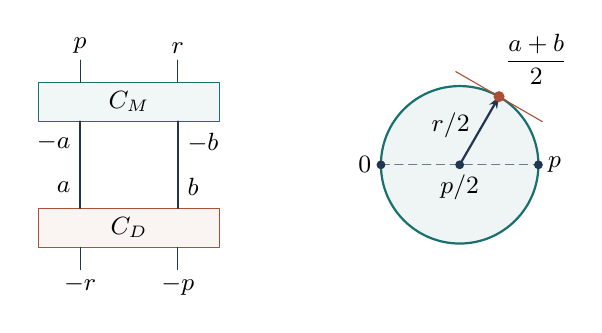
\begin{tikzpicture}[font=\small,line cap=round,line join=round]
 \begin{scope}[xshift=-2.2cm]
  \node[draw=sea,fill=sea!6,minimum width=2.3cm,minimum height=5mm] (M) at (0,.8) {$C_M$};
  \node[draw=rust,fill=rust!6,minimum width=2.3cm,minimum height=5mm] (D) at (0,-.8) {$C_D$};
  \draw[ink] (-.62,1.33)--(-.62,1.05) (.62,1.33)--(.62,1.05);
  \node[above] at (-.62,1.29) {$p$};
  \node[above] at (.62,1.29) {$r$};
  \draw[thick,ink] (-.62,.55)--(-.62,-.55) (.62,.55)--(.62,-.55);
  \node[left] at (-.62,.28) {$-a$};
  \node[right] at (.62,.28) {$-b$};
  \node[left] at (-.62,-.28) {$a$};
  \node[right] at (.62,-.28) {$b$};
  \draw[ink] (-.62,-1.05)--(-.62,-1.33) (.62,-1.05)--(.62,-1.33);
  \node[below] at (-.62,-1.29) {$-r$};
  \node[below] at (.62,-1.29) {$-p$};
 \end{scope}
 \begin{scope}[xshift=1.0cm]
  \fill[sea!7] (1,0) circle (1cm);
  \draw[thick,sea] (1,0) circle (1cm);
  \draw[densely dashed,ink!65] (0,0)--(2,0);
  \draw[-{Stealth[length=1.5mm]},thick,ink] (1,0)--(1.5,.866);
  \node[left] at (1.25,.50) {$r/2$};
  \fill[ink] (0,0) circle (1.6pt) (1,0) circle (1.6pt) (2,0) circle (1.6pt);
  \node[left] at (0,0) {$0$};
  \node[below] at (1,0) {$p/2$};
  \node[right] at (2,0) {$p$};
  \draw[rust] (.95,1.184)--(2.05,.548);
  \fill[rust] (1.5,.866) circle (2pt);
  \node[above right,inner sep=2.5pt] at (1.48,.92) {$\displaystyle\frac{a+b}{2}$};
 \end{scope}
\end{tikzpicture}
\caption{A boundary force on the two-phase contraction lifts with opposite
signs on each internal wire (left). The three-leg rank bounds put both
internal vectors $a,b$ in the disk with diameter $[0,p]$ (right).
Their midpoint is $p/2+r/2$ on the supporting tangent, so both vectors
coincide with it.}
\label{geo:force-figure}
\end{figure}

It remains to turn this constraint on the intermediate legs into
distances at an arbitrary placement. Let $M_j\in\mathcal A$ be the
first matrices on the chosen subsequence. Move the input copies of $x,y$
out to $Rp,Rr$ while leaving the output copies at $A',B'$. For each
fixed $R>0$ the limiting first-phase forces give
\[
 \liminf_{j\to\infty}\frac{P_{M_j}(Rp,Rr,A',B')}{m}
       \ \ge\ 2R-\tfrac12(p+r)\cdot(A'+B').
\]
We can implement the move by copying each matched pair to the new
input site and then erasing its old input copy with an all-ones
covector. By \eqref{geo:copy}, the increase in price divided by $m$
is at most
\[
 2R-\tfrac12\bigl(p\cdot(A+A')+r\cdot(B+B')+
                         |A-A'|+|B-B'|\bigr)+o(1),
\]
using $|Rp-X|=R-p\cdot X+o(1)$ as $R\to\infty$. Subtracting the
cost of the move and letting $R\to\infty$ gives
\[
 \sup_{M\in\mathcal A}\frac{2P_M(A,B,A',B')}{m}
 \ \ge\ |A-A'|+|B-B'|+p\cdot(A-B')+r\cdot(B-A').
\]
The first two lengths come from the two pairs of matching labels in
the copying inequality. Maximizing over the independent choices of
$p,r$ gives the two crossed lengths and proves \eqref{geo:four-legs}.
The first matrices used to bound the supremum may depend on $p,r$.
\end{proof}

\begin{proof}[Proof of Theorem~\ref{geo:saturation}]
The case $N=1$ has price zero at every placement. For $N\ge2$ the
upper bound is \eqref{geo:upper}. In Proposition~\ref{geo:first-phase}
the two same-label distances on a rectangle are $L$ and the two
crossed distances are $D$. Its lower bound is therefore $m(L+D)$.
Lemma~\ref{geo:swap} applies with the singleton $\mathcal A=\{F_G\}$.
\end{proof}

\begin{remark}[Convex quadrilaterals]\label{geo:quadrilateral}
The same price computation determines $P_{F_G}$ on four sites in
convex position. If $d_1,d_2$ are the lengths of their hull diagonals,
then
\[
 P_{F_G}(A,B,A',B')
   =\tfrac m2\bigl(|A-A'|+|B-B'|+d_1+d_2\bigr).
\]
The intersection $O$ of the hull diagonals gives an upper bound by
supplying the common labels on $A,A',O$ and $B,B',O$. The four
distances from the vertices to $O$ sum to $d_1+d_2$.
If both diagonals join unlike labels, exchanging the two copies of
one label if necessary places their lengths in the last two terms
of \eqref{geo:four-legs}. Exchanging these copies preserves the tensor
under the coordinate identification of the basis with its dual.
If the diagonals join like labels, their two wires give the tensor
up to nonzero character weights, and both wires pass through $O$.
The copying theorem then preserves their full price under reweighting.
\end{remark}


\section{The lower bound for independent transforms}\label{bch:proof:section}

A circuit can mix coordinates from all its input signals in a single
state. A low-rank correction to its output can do the same. To obtain
a bound proportional to the number of signals, we test the input
coordinates and Fourier outputs of each signal together. The rectangle
calculation in Section~\ref{geo:section} gives a lower bound on this
test even after a projection removes a small fraction of the dimensions.
We then show that a projection of the whole batch must preserve most
of these individual tests. Throughout the proof we work over the
algebraic closure $k$ of the coefficient field.

\subsection{A character table after projection}

For a matrix $U$ with columns $u_j$, its \emph{list tensor} is
$\mathcal D(U)=\sum_j u_j\otimes e_j\otimes e_j$. The label $j$ is
recorded twice so that we may place it at both ends of one side of a
rectangle. Put the vector leg at the center $O$ and the label legs on
the left side as in Figure~\ref{geo:rectangle-figure}. Write $V_-(U)$
for the spectral value $\Phi_S(\mathcal D(U))$ at these three sites
and $V_+(U)$ for its counterpart on the right. Set $V_\pm(0)=0$.
For a transform of order $N$, we use width one and height $L=3/\sqrt m$,
where $m=\log_2 N$. The triangle and rectangle have semiperimeters
\[
 \delta=\tfrac12\bigl(L+\sqrt{1+L^2}\bigr),
 \qquad \Delta=1+L .
\]
For the matrix $U=[I_N\ H]$ the list contains the coordinate vectors
and the columns of a character table. Its value on either triangle
is at most $2N$, the cost in spectral value of supplying the column
label itself. The next estimate retains nearly this value on a single
triangle after projection.

\begin{lemma}[Testing a projected character table]\label{bch:projected-list}
There is an absolute $N_0$ with the following property. Let $H$ be
the character table, in symmetric character coordinates, of a split
finite abelian group of order $N\ge N_0$ invertible in $k$. Put
$U=[I_N\ H]$ and $\varepsilon=2^{-100}$. Every linear map $Q$ on
the vector leg of rank at least $(1-\varepsilon)N$ satisfies
$V_-(QU)\ge1.8N$.
\end{lemma}

\begin{proof}
Choose a cyclic decomposition of the group and a primitive root on
each axis. The resulting symmetric bicharacter gives $H^{\mathsf T}=H$
and $H^{\mathsf T}H=NP$, where $P$ represents $g\mapsto-g$.
Put one copy of $\mathcal D(U)$ on each triangle and contract their
vector legs at $O$ by the usual bilinear pairing. The rectangle tensor
that remains is specified by the Gram matrix
\[
 U^{\mathsf T}U=\begin{pmatrix} I_N&H\\ H&NP\end{pmatrix}.
\]
The two diagonal blocks together have rectangle value $2N$, since
they supply a single common label up to local permutations and
nonzero scalings. The two off-diagonal blocks form a direct sum of
character-table tensors. Theorem~\ref{geo:saturation} gives each of
these price $2\delta m$ and hence rectangle value $2^{2\delta m/\Delta}$.
Subtracting the diagonal blocks from the Gram tensor and applying
\eqref{geo:sum} bounds the Gram value from below. On the other hand,
contracting at $O$ gives a price at most the sum of the two triangle
prices, by compatibility under insertion of trivial legs. Together
these estimates give
\[
   \bigl(V_-(U)V_+(U)\bigr)^{\delta/\Delta}
       \ge 2\,2^{2\delta m/\Delta}-2N .
\]
Put $a=m(2\delta-\Delta)/\Delta$. As each triangle value is at most
$2N$, the value on either one divided by $N$ is at least
$[2(1-2^{-a})]^{\Delta/\delta}/2$. The choice of height makes the
curvature term $a$ tend to $9/2$, while $\Delta/\delta\to2$.
The limiting lower bound is $2(1-2^{-9/2})^2>1.82$.

It remains to control the part removed by $Q$. Choose a linear map $E$
such that $EQ$ projects onto a complement to $\ker Q$ and put
$W=(I-EQ)U$. If its rank $r$ is positive, place a supplier halfway
from $O$ to the midpoint of the left side. A common label of size
$2N$ at the supplier and both left corners specifies a column of $W$.
Carry its coordinates in a basis of $\operatorname{im}W$ along a wire
of length $1/4$ and dimension $r$ to $O$. The triangle used by the
common label has semiperimeter
$\tau=L/2+\sqrt{1/16+L^2/4}$. Thus
\[
 \delta\log V_-(W)
 \le \tau\log(2N)+\tfrac14\log r
 \le \delta m+\tfrac92+\tau-25 .
\]
The last inequality uses $r\le2^{-100}N$ and
$\tau+1/4-\delta\le L^2/2=9/(2m)$. Since $\delta\to1/2$ and
$\tau\to1/4$, this gives $V_-(W)<0.01N$ for all sufficiently
large $N$. The estimate also holds when $r=0$. Now $U=EQU+W$,
so subadditivity and restriction at $O$ imply
$V_-(U)\le V_-(QU)+V_-(W)$.
\end{proof}

\subsection{Removing a rank correction from the whole batch}

Set $V=V_-$ and $p=L/\delta\in(0,1)$. We can annihilate a global
rank correction by projecting the output coordinates. This projection
may mix the blocks of independent signals. The next lemma extracts
one projection per block without increasing their total rank loss
or their total list value.

\begin{lemma}[A row quotient across independent lists]\label{bch:quotient-test}
Let $A=\bigoplus_i U_i$ have $h$ rows, in blocks of sizes $n_i$.
Suppose $A$ is in the closure of sums of a matrix of rank at most $r<h$
and a matrix with at most $T$ nonzero entries. There are $n_i$-square
matrices $Q_i$ such that
\[
 \sum_i(n_i-\operatorname{rank} Q_i)\le r,\qquad
 \sum_i V(Q_iU_i)\le h(T/h)^p .
\]
\end{lemma}

\begin{proof}
For an actual sum $B+P$, choose $h-r$ independent row vectors
annihilating $B$ and form the matrix $Q$ with these rows. Decompose
$QP$ into contributions from the rows of $P$. The contribution of
row $i$ has fixed vector leg, the $i$th column of $Q$, and two copies
of a label ranging over the $t_i$ nonzero entries of that row.
A wire of dimension $t_i$ and length $L$ between the two label
sites supplies this contribution, including its coefficients by a local
map. Its list value is at most $2^{L\log(t_i)/\delta}=t_i^p$ when
$t_i>0$, and zero when $t_i=0$. Subadditivity and concavity give
\[
 V(Q(B+P))=V(QP)
    \le\sum_i t_i^p\le h(T/h)^p .
\]

The annihilator can vary as $B+P$ approaches a border point. To see
that some quotient still gives the same bound there, consider the
Grassmannian of $(h-r)$-dimensional subspaces of $(k^h)^*$.
On each standard chart a basis matrix $Q$ depends regularly on the
subspace. For a matrix $M$, the condition $V(QM)\le h(T/h)^p$ is closed
by Theorem~\ref{geo:spectrum}, and changing the basis of the rows of
$Q$ preserves the list value. The chart conditions therefore define
a closed incidence set in the product of the Grassmannian with matrix
space. The Grassmannian is projective, so the image in matrix space
is closed. In particular the target $A$ admits such a $Q$.

At the block-diagonal target, put the rows of $Q$ in echelon form
and insert each into the row position of its pivot in a square matrix,
filling the other rows with zeros. This replacement preserves the list
value by local maps in both directions. The resulting matrix, still
denoted by $Q$, is upper triangular. Each pivot contributes one to
the rank of its diagonal block $Q_i=Q_{ii}$, so
$\sum_i\operatorname{rank}Q_i\ge h-r$.

The $(i,j)$ block of $QA$ is $Q_{ij}U_j$. Scale the vector block $i$
by $z^{-i}$ and the label block $j$ at one of its two sites by $z^j$.
These local maps are invertible for $z\ne0$. Each surviving block
acquires a factor $z^{j-i}$ with nonnegative exponent. At $z=0$ only
the diagonal blocks remain (Figure~\ref{bch:quotient-figure}). Closed
sublevels and additivity on direct sums give
$\sum_i V(Q_iU_i)\le V(QA)$.
\end{proof}

\begin{figure}[htb]
\centering
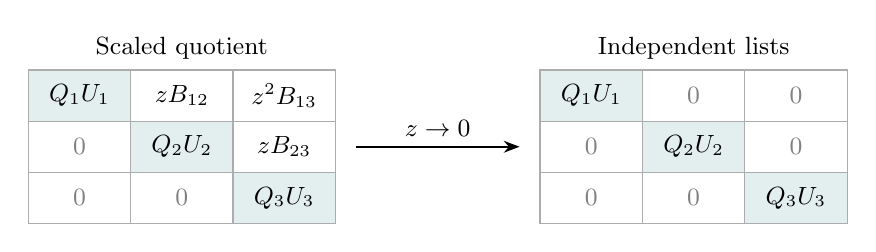
\begin{tikzpicture}[x=1.3cm,y=.65cm,font=\small]
  \foreach \off in {0,5} {
    \foreach \i in {0,1,2} {
      \fill[sea!12] (\off+\i,-\i) rectangle (\off+\i+1,-\i-1);
    }
    \draw[gray!65] (\off,0) rectangle (\off+3,-3);
    \foreach \i in {1,2}
      \draw[gray!65] (\off+\i,0)--(\off+\i,-3) (\off,-\i)--(\off+3,-\i);
    \foreach \i/\b in {0/1,1/2,2/3}
      \node at (\off+\i+.5,-\i-.5) {$Q_{\b}U_{\b}$};
  }
  \node at (1.5,.43) {Scaled quotient};
  \node at (6.5,.43) {Independent lists};
  \node at (1.5,-.5) {$zB_{12}$}; \node at (2.5,-.5) {$z^2B_{13}$};
  \node at (2.5,-1.5) {$zB_{23}$};
  \foreach \x/\y in {.5/-1.5,.5/-2.5,1.5/-2.5,5.5/-1.5,5.5/-2.5,6.5/-2.5,6.5/-.5,7.5/-.5,7.5/-1.5}
    \node[gray] at (\x,\y) {$0$};
  \draw[-{Stealth[length=2mm]},thick] (3.2,-1.5)--(4.8,-1.5)
    node[midway,above] {$z\to0$};
\end{tikzpicture}
\caption{An echelon quotient of three independent lists. The mixed
blocks $B_{ij}=Q_{ij}U_j$ vanish under scaling. Each pivot survives
in a shaded diagonal block, and the three surviving list values add.}
\label{bch:quotient-figure}
\end{figure}

\subsection{Repeating the transfer on a time coordinate}

The quotient test charges independent Fourier lists. To turn the number
of states into a rank budget for that test, we run the same transfer on
$d$ time coordinates. Making the time shift nilpotent changes
one column in a suitable basis. This costs at most one unit of rank
per state and truncates every dependency path at depth $d$, so each
row of the resulting transfer has small support.
For related time expansions of feedback circuits see
\cite[Sections~5--6]{FiniteFourier}.

\begin{lemma}[Time expansion]\label{bch:time-expansion}
Let $M\in\mathcal C_s(h)$ be the transfer of a binary linear system
and let $d\ge1$. Then $I_d\otimes M$ belongs to the closure of sums of
a matrix of rank at most $s$ and a matrix with at most $d2^{d-1}$
nonzero entries per row.
\end{lemma}

\begin{proof}
Write the state equations as $v=Cv+Ax$. Uniqueness at $x=0$ implies
that $I-C$ is invertible. Pad with zero states to obtain exactly $s$
states. Replace each state by $d$ copies, writing $C'=C\otimes I_d$
and $A'=A\otimes I_d$, and after each state apply a shift on its
$d$ time values. Consider two choices for this shift. First take
$R=I_d+D$, where $D$ sends $e_i$ to $e_{i+1}$ and kills $e_d$.
The vectors $e_1,Re_1,\ldots,R^{d-1}e_1$ form a basis in every
characteristic, by triangularity. In this basis take $R_0$ to act as
$R$ on the first $d-1$ vectors and to kill the last. Then $R_0^d=0$
and $\operatorname{rank}(R-R_0)=1$.

For $S=R$ or $R_0$, put $Z_S=I_s\otimes S$. The input-to-state
map $V_S$ solves $V_S=Z_S(C'V_S+A')$. For $R$, the equations are
triangular in the original time coordinates with invertible diagonal
blocks $I-C$. For $R_0$, $Z_{R_0}C'=C\otimes R_0$ is nilpotent.
Subtracting the two systems gives
\[
 (I-Z_R C')(V_R-V_{R_0})
       =(Z_R-Z_{R_0})(C'V_{R_0}+A').
\]
The right side has rank at most $s$, one per state. The same rank
bound holds after the output readout, since any direct readout of an
input is the same in both transfers.

In the transfer for $R_0$, any path visiting $d$ states has zero
contribution. Unroll a single readout into a binary dependency tree
truncated after $d-1$ state expansions along each path. At most
$2^{d-1}$ leaves can be original input coordinates. Each such coordinate
carries $d$ time values, so the row has at most $d2^{d-1}$ nonzeros.

In the original time basis the transfer for $R$ is lower triangular
in time with diagonal blocks $M$. Multiply each output time block $i$
by $t^{i-1}$ and each input time block $j$ by $t^{1-j}$. For $t\ne0$
this preserves rank and support. Sending $t$ to zero removes the
strictly lower blocks and leaves $I_d\otimes M$ in the claimed closure.
\end{proof}

\subsection{Comparing the two budgets}

\begin{proof}[Proof of Theorem~\ref{bch:uniform-robust}]
Let $h=JN$, $m=\log_2 N$, $d=\lceil\sqrt m/8\rceil$, and $h_d=dh$.
In symmetric character coordinates the inverse transform differs from
the forward transform by a permutation and a nonzero scalar. Such
permutations and scalings preserve all three budgets, so take each
block to be a forward transform $H_j$.

Suppose the target is in the geometric border of $M+B+Z$ as in
Theorem~\ref{bch:uniform-robust}. For an actual sum, apply
Lemma~\ref{bch:time-expansion} to $M$ and repeat $B,Z$ on the $d$
time coordinates. Transpose the result and adjoin $I_{h_d}$ as
input columns. Transposition preserves the total number of nonzero
entries, and the identity adds $h_d$ entries. This operation on
$M+B+Z$ is affine in the sum, so it maps the joint border into
the closure of rank-plus-sparse sums with the same budgets. At the
target the resulting list is, up to permutations, the direct sum of
$d$ copies of each $[I_N\ H_j]$. The rank and total support budgets are
\[
 r=s+d\lfloor\beta h\rfloor,\qquad
 T=h_d(1+d2^{d-1})+d\lfloor\eta h\,2^{\sqrt m/8}\rfloor .
\]

Take $\beta=\varepsilon/400$ and $\eta\le1$. If
$s\le\varepsilon h_d/400$, the sum of rank deficits in
Lemma~\ref{bch:quotient-test} is at most $\varepsilon h_d/200$.
At least a fraction $199/200$ of the $Jd$ blocks therefore retain
rank at least $(1-\varepsilon)N$. For all sufficiently large $N$,
Lemma~\ref{bch:projected-list} gives total list value at least
$1.8(199/200)h_d>1.79h_d$. But Lemma~\ref{bch:quotient-test}
bounds it by $h_d(T/h_d)^p$, where
\[
 (T/h_d)^p\le (1+d2^{d-1}+2^{\sqrt m/8})^p
       \longrightarrow 2^{3/4}<1.79 .
\]
Indeed $p\sqrt m\to6$ and $d/\sqrt m\to1/8$. This contradiction
gives $s>\varepsilon h\sqrt m/3200$ uniformly in $J$ and the field.

For the finitely many smaller orders, we find two disjoint sets of
input columns on which many output rows still have full rank. In each
group choose a cyclic factor of order $e\ge2$ and let
$\ell=\lfloor e/2\rfloor$. The first $\ell$ exponent rows paired
with either of two disjoint sets of $\ell$ nodes give invertible
Vandermonde minors. Tensoring with the other cyclic factors and taking
the direct sum over the groups gives a common set of $u\ge h/3$
rows with full row rank on each of two disjoint column sets.

For any circuit readout, the direct-input part of each selected row
misses at least one of the two column sets. A state readout has zero
direct-input part and misses both. On at least $u/2$ rows one common
column set is missed. The transfer restricted to these rows and that
column set has rank at most $s$ by factorization through the states.
The corrections add at most $\beta h+|\operatorname{supp} Z|$ to
the rank. There are finitely many choices of rows and column set at
each size, so the union of these rank conditions is closed. Full row
rank at the target now gives $u/2\le s+\beta h+\eta h2^{\sqrt m/8}$.
Shrink $\eta$ once so that $\beta+\eta 2^{\sqrt m/8}\le1/12$ for
every order in this finite range. Then $s\ge h/12$. Decreasing the
absolute constant in the lower bound proves the assertion at all orders.
An acyclic circuit of size $s$ is a uniquely solvable system with $s$
states. Taking $B=Z=0$ gives the lower bound of Theorem~\ref{thm:main}.
\end{proof}


\part{An exact algorithm on prime tensor powers}\label{part:finite}
\section{Prediction and exact spectral repair}\label{sec:repair}

The Fourier construction in Section~\ref{sec:prime-kernel} expresses
a large transform as a product of \(m\) commuting operators. Applying
them one at a time would cost \(m\) stages. In a common eigenbasis their
product acts by a single scalar at each frequency, but changing to that
basis on every input row would itself be expensive. We use a low-degree
predictor on a batch of independent rows. At each frequency it is exact
on almost all rows, and a small number of linear checks recovers the
product on the whole batch. The exceptional rows may change from one
frequency to the next.

Let \(\ell\) be prime, let \(\zeta\) be a primitive complex \(\ell\)-th
root of unity, and set \(R_\ell=\mathbb Z[1/\ell,\zeta]\). A row is an
array indexed by a finite set, with coefficients in a commutative
\(R_\ell\)-algebra. Suppose that one invertible change of coordinates
\(\mathcal S\) diagonalizes \(Q_1,\ldots,Q_m\) on this array. At frequency
\(\nu\), operator \(Q_j\) has multiplier \(\zeta^{k_j(\nu)}\), and the
exponents \(k_j(\nu)\) are given. Write \(F=\prod_{j=1}^m Q_j\).

We count two operations on a batch of \(W\) rows. A \emph{pencil stage}
combines the query powers with scalar matrices acting on the row index,
\begin{equation}\label{eq:repair-pencil}
  A_0\otimes I+\sum_{j=1}^m\sum_{a=1}^{\ell-1}A_{ja}\otimes Q_j^a,
       \qquad A_0,A_{ja}\in\operatorname{Mat}_{W\times W}.
\end{equation}
A \emph{spectral table on \(h\) rows} takes \(h\) forward conversions by
\(\mathcal S\), applies one prescribed \(h\times h\) scalar matrix at
each frequency, and takes \(h\) inverse conversions. Pointwise linear
maps combine rows at the same ordinary index. A pencil stage can
contain all \(m\) queries. The next section bounds the cost of executing
such a stage in the Fourier construction.

\needspace{4\baselineskip}
\begin{theorem}[Simultaneous spectral repair]\label{thm:repair}
For every \(m\ge2\) there are a positive batch width \(W\) and a finite
free cyclotomic extension of \(R_\ell\), depending only on \(\ell,m\),
over which a program computes \(F\) on \(W\) independent rows. It uses
\(O_\ell(\sqrt{m\log(2m)})\) pencil stages, pointwise linear maps and
one spectral table on \(2s\) rows, with \(s\le W/(2m^3)\). The table
thus uses at most \(4s\) full row conversions. Its matrix at frequency
\(\nu\) depends only on \((k_j(\nu))_{j=1}^m\). All row matrices and the
finite list of spectral matrices are effectively constructible for fixed
\(\ell,m\). The identities specialize to any commutative \(R_\ell\)-algebra
after base change along the finite free extension.
\end{theorem}

\subsection{Predicting the product from an integer count}

Assign each row a shift \(\beta\in(\mathbb Z/\ell\mathbb Z)^m\), using
every shift equally often. At a fixed \(\nu\), write \(q_j=\zeta^{k_j(\nu)}\)
and \(z=\prod_jq_j\) for the desired multiplier. Let \(b_j\) be the least
nonnegative residue of \(k_j(\nu)+\beta_j\), and put \(c=\sum_j b_j\)
as an ordinary integer. On a row with shift \(\beta\), it suffices to
predict \(\zeta^{c-\sum_j\beta_j}=z\). Varying the shift makes the digits
\(b_j\) uniform and independent at every fixed frequency.

For three binary queries, for example, \(c\) is the Hamming weight of
\(k+\beta\). On the window \(1\le c\le2\), the linear predictor
\((-1)^{|\beta|}(2c-3)\) gives the target sign \((-1)^{|k|}\).
The two shifts outside the window are \(000,111\) at \(k=000\), but
\(001,110\) at \(k=001\).

In general, let \(r\) be the least integer with \(2^r\ge2m\). Set
\[
 \mu=m(\ell-1)/2,\qquad B=(\ell-1)\lceil\sqrt{2mr}\rceil,\qquad
 u=\lfloor\mu-B\rfloor,\quad v=\lceil\mu+B\rceil .
\]
These endpoints are computable by integer arithmetic. Hoeffding's
inequality \cite[Theorem~2]{hoeffding} bounds the fraction of rows
outside this window at each frequency,
\[
 \Pr_\beta[c\notin[u,v]]
    \le 2\exp\!\left(-\frac{2B^2}{m(\ell-1)^2}\right)
    \le \frac{1}{2m^3}.
\]
The predictor will have degree at most the width \(D=v-u\). We use
integral interpolation so that its coefficients also make sense in
positive characteristic.

\begin{lemma}[Integral interpolation on the count]\label{lem:count-predict}
For each shift \(\beta\) there is a polynomial \(P_\beta\) over
\(R_\ell\), of degree at most \(D=v-u\) in the variables representing
the query powers \(Q_j^a\), \(1\le a<\ell\). At each frequency with
\(c\in[u,v]\) this polynomial equals the multiplier of \(F\).
\end{lemma}
\begin{proof}
The indicator for the event \(b_j=b\) is affine-linear in the query powers,
\[
 I_{j,b}=\frac1\ell\sum_{a=0}^{\ell-1}\zeta^{a(\beta_j-b)}q_j^a.
\]
For \(h>0\), the coefficient of \(T^h\) in \((1+T)^{b_j}\) is thus
represented by \(\sum_{b=0}^{\ell-1}\binom bh I_{j,b}\). Use \(1\)
for the constant coefficient. In the formal expansion
\[
 L_h=[T^h](1+T)^{-u}\prod_{j=1}^m(1+T)^{b_j}
\]
each term uses a positive power of \(T\) from at most \(h\) query
factors. It follows that \(L_h\) has a representation of degree at
most \(h\) in the query powers. The fixed series \((1+T)^{-u}\) has
integer coefficients.

Now take
\[
 P_\beta=\zeta^{\,u-\sum_j\beta_j}
                \sum_{h=0}^{D}(\zeta-1)^h L_h .
\]
On the window, \(0\le c-u\le D\). The truncated sum therefore evaluates
the whole polynomial \((1+T)^{c-u}\) at \(T=\zeta-1\) and returns
\(\zeta^{c-\sum_j\beta_j}=z\) after scaling.
\end{proof}

\subsection{Evaluating a predictor on independent rows}

A polynomial of degree \(D\) can have many monomials. To evaluate it in
\(O_\ell(D)\) pencil stages, increase the batch width and express the
polynomial times the identity as a power of one matrix of affine-linear
forms. The identity factor ensures that every coordinate of the matrix
holds an independent input.

Childs studied such linearizations of forms through generalized Clifford
algebras \cite{childs}. For homogeneous forms over a field with a
primitive root of the required order, see Bl\"aser, Eisenbud and
Schreyer \cite[Theorem~2.1]{ulrichcomplexity}. We give the construction
over a localized cyclotomic ring to obtain a pencil that specializes in
every characteristic allowed here.

\begin{lemma}[Matrix evaluation of a polynomial]\label{lem:matrix-root}
Let \(p\) be a polynomial of degree at most \(b\) over \(R_\ell\), where
\(b=\ell^a\ge2\). If \(\xi\) is a primitive \(b\)-th root of unity,
there is a square matrix \(L\) of affine-linear forms over
\(R_\ell[\xi]\) such that \(L^b=pI\).
\end{lemma}
\begin{proof}
Write \(p=\sum_{i=1}^h\prod_{r=0}^{b-1}\lambda_{ir}\), padding each
monomial with constant factors so that every \(\lambda_{ir}\) is
affine-linear. On the \(i\)-th copy of a free module with basis
\(e_0,\ldots,e_{b-1}\), put
\[
 S_i e_r=\lambda_{ir} e_{r+1\bmod b},\qquad Z e_r=\xi^r e_r .
\]
Then \(S_i^b=(\prod_r\lambda_{ir})I\) and \(ZS_i=\xi S_i Z\).
On the tensor product of the \(h\) modules take
\[
 L=\sum_{i=1}^h Z^{\otimes(i-1)}\otimes S_i\otimes I^{\otimes(h-i)} .
\]
Each summand \(V\) satisfies \(VU=\xi UV\) for \(U\) the sum of the
preceding summands. Potter's identity \cite{potter} gives
\((U+V)^b=U^b+V^b\) over the complex numbers. To see why it survives
specialization, order the factors in the expansion of \((U+V)^b\)
using \(VU=\xi UV\). The coefficient of \(U^{b-r}V^r\) is the
Gaussian binomial polynomial
\[
 \genfrac{[}{]}{0pt}{}{b}{r}_{\!X}
     =\prod_{j=1}^r\frac{1-X^{b-j+1}}{1-X^j}
\]
evaluated at \(X=\xi\), by the recurrence obtained on multiplying the
ordered expansion by \(U+V\). For \(0<r<b\) the denominators are
nonzero at a complex primitive \(b\)-th root, while the numerator
contains \(1-X^b\). Thus \(\Phi_b(X)\) divides the Gaussian binomial
in \(\mathbb Z[X]\). Every mixed coefficient vanishes over \(R_\ell[\xi]\)
and under any specialization. The \(b\)-th power of \(L\) is therefore
the sum of the \(b\)-th powers of its summands, which is \(pI\).
\end{proof}

Take \(b\) to be the least power of \(\ell\) at least \(\max(2,D)\).
Apply Lemma~\ref{lem:matrix-root} to every \(P_\beta\), padding the
monomial lists by zero terms to obtain matrices of one dimension.
Give each shift a block of that many independent rows. On the direct
sum of the blocks, \(b\) repetitions of one pencil stage compute a
predictor \(P\). At each frequency \(P\) is diagonal in the individual
rows. Write \(p_i\) for its multiplier on row \(i\). The exponent tuple
specifies the set \(J=J(\nu)\) of rows outside the window. It has size
at most \(s=\lfloor W/(2m^3)\rfloor\) and contains every row where
\(p_i\ne z\).

\subsection{Sending the error through a small spectral table}

At each frequency the prediction error has at most \(s\) known
positions. We can recover their values from \(s\) linear checks.
Returning them to the correct ordinary rows poses a second problem.
The set of destination rows changes with the frequency. Our lift
from the inverse-transformed rows uses a fixed row matrix, which acts
identically at every frequency. To make that lift work, we replace the
predictor by a polynomial whose error vanishes to second order at the
target multiplier.

\begin{lemma}[Full-rate Hermite repair]\label{lem:hermite-repair}
Work over a commutative ring in which \(\ell\) is invertible and there
are \(W\) elements with pairwise unit differences. Suppose that at each
frequency \(F\) has the same multiplier \(z\) on all rows, with
\(z^\ell=1\), and that \(P\) has known row multipliers \(p_i\) agreeing
with \(z\) off a known set \(J\) of size at most \(s\). Then \(F\) on
\(W\) independent inputs can be computed with at most \(\ell+2\)
applications of \(P\), one spectral table on \(2s\) rows and
pointwise linear maps.
\end{lemma}
\begin{proof}
If \(s=0\), \(P\) already gives \(F\). Otherwise, choose the \(s\times W\)
Vandermonde matrix \(H\) with powers \(0,\ldots,s-1\) on the given
nodes. Over a field these are the parity checks of a generalized
Reed--Solomon code \cite{reedsolomon}. For \(j=|J|\le s\), the first
\(j\) rows of the column submatrix \(H_J\) give a Vandermonde
determinant that is a unit. Hence \(H_J\) has a left inverse and
\(H_J^{\mathsf T}\) a right inverse.

On the batch \(X\), form \(PX\) and convert the \(2s\) check rows
\(HPX,HX\) to spectral coordinates. At one frequency the error vector
\(e\) satisfies
\[
 e_i=(p_i-z)\widehat X_i,\qquad
 He=H\widehat{PX}-zH\widehat X.
\]
The left inverse of \(H_J\) recovers \(e_J\) from \(He\).

To correct the output, first replace the predictor by the polynomial
\(g(P)\), where
\[
 g(y)=y-\ell^{-1}y(y^\ell-1).
\]
At every allowed \(z\), \(g(z)=z\) and \(g'(z)=0\). Dividing by the
monic polynomial \((y-z)^2\) gives
\(g(y)-z=(y-z)^2D_z(y)\) over the ring. Use the right inverse of
\(H_J^{\mathsf T}\) to choose an \(s\)-vector \(a\), linear in \(e_J\),
satisfying
\[
 (H^{\mathsf T}a)_i=D_z(p_i)e_i\qquad(i\in J).
\]
The table returns the pair \(a,za\). After inverse conversion and
pointwise multiplication by \(H^{\mathsf T}\), these are ordinary
rows \(Z,FZ\) with \(\widehat Z=H^{\mathsf T}a\)
(Figure~\ref{fig:repair-table}). Output \(g(P)X-PZ+FZ\).
Its error on row \(i\) at this frequency is
\[
 (p_i-z)\bigl(D_z(p_i)e_i-\widehat Z_i\bigr).
\]
The second factor vanishes on \(J\), and the first vanishes outside
\(J\). Thus the entire batch is correct. We reuse the initial \(PX\)
to form \(P^{\ell+1}X\) for \(g(P)X\), and apply \(P\) once more
to \(Z\). This totals \(\ell+2\) predictor applications.
\end{proof}

\begin{figure}[!htb]
\centering
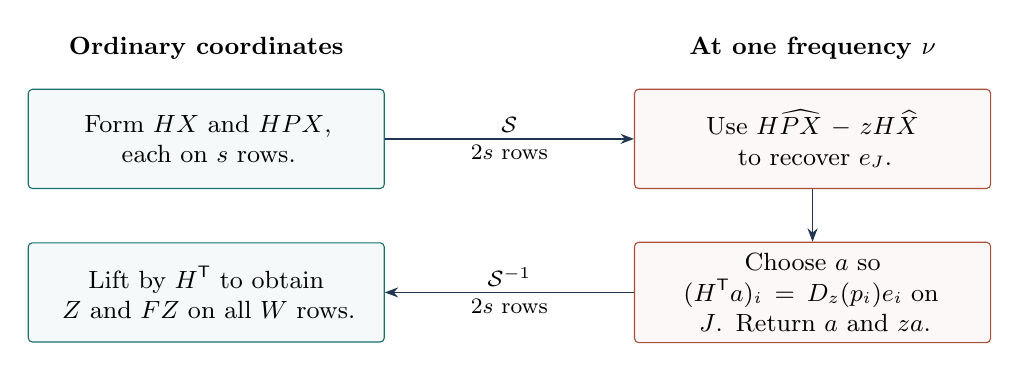
\begin{tikzpicture}[
  font=\small,align=center,
  repair box/.style={draw=#1,fill=#1!4,rounded corners=1.5pt,
    inner xsep=6pt,inner ysep=4pt,text width=4.1cm,minimum height=1.26cm},
  repair path/.style={-{Stealth[length=1.7mm]},draw=ink,line width=.55pt},
  repair note/.style={font=\footnotesize,inner sep=2pt,align=center}
]
\node[anchor=south,font=\small\bfseries] at (0,.89) {Ordinary coordinates};
\node[anchor=south,font=\small\bfseries] at (7.7,.89) {At one frequency \(\nu\)};
\node[repair box=sea] (checks) at (0,0)
  {Form \(HX\) and \(HPX\),\\ each on \(s\) rows.};
\node[repair box=rust] (recover) at (7.7,0)
  {Use \(H\widehat{PX}-zH\widehat X\)\\ to recover \(e_J\).};
\node[repair box=rust] (coeffs) at (7.7,-1.95)
  {Choose \(a\) so \((H^{\mathsf T}a)_i=D_z(p_i)e_i\) on \(J\). Return \(a\) and \(za\).};
\node[repair box=sea] (lift) at (0,-1.95)
  {Lift by \(H^{\mathsf T}\) to obtain\\ \(Z\) and \(FZ\) on all \(W\) rows.};
\draw[repair path] (checks.east) -- node[repair note,above]{\(\mathcal S\)}
   node[repair note,below]{\(2s\) rows} (recover.west);
\draw[repair path] (recover.south) -- (coeffs.north);
\draw[repair path] (coeffs.west) -- node[repair note,above]{\(\mathcal S^{-1}\)}
  node[repair note,below]{\(2s\) rows} (lift.east);
\end{tikzpicture}
\caption{Repairing the predictor on \(W\) independent inputs. Only
\(2s\) rows cross into spectral coordinates and back. The table
prescribes the lifted correction on \(J(\nu)\). At every other row
\(p_i=z\), so subtracting \(PZ-FZ\) has no effect there.}
\label{fig:repair-table}
\end{figure}


\begin{proof}[Proof of Theorem~\ref{thm:repair}]
With \(W\) fixed, choose \(t\ge1\) so that \(\ell^t\ge W\) and
\(b\mid\ell^t\). Take a primitive \(\ell^t\)-th root \(\eta\) with
\(\eta^{\ell^{t-1}}=\zeta\). The cyclotomic degrees give the basis
\(1,\eta,\ldots,\eta^{\ell^{t-1}-1}\) for
\(R'=\mathbb Z[1/\ell,\eta]\) over \(R_\ell\). This ring contains the
matrix coefficients and supplies \(W\) Vandermonde nodes from the
powers of \(\eta\). For the quotient \(\rho\) of any two distinct
nodes, of order \(\ell^h\), the product of \(1-\rho^j\) over \(j\)
prime to \(\ell\) modulo \(\ell^h\) is \(\Phi_{\ell^h}(1)=\ell\).
Each factor is a unit, so the nodes have pairwise unit differences.

Each predictor application takes \(b\) pencil stages. Hence
Lemma~\ref{lem:hermite-repair} uses at most
\((\ell+2)b=O_\ell(\sqrt{m\log(2m)})\) stages and converts \(2s\)
rows in each direction. The bases, inverses and finite list of tables
can be constructed in \(R'\) from \(\ell^{-1}\) and the indicated
roots. These ring identities give the asserted program after base
change to every commutative \(R_\ell\)-algebra.
\end{proof}

The same construction applies to swaps of address fields. The following
form of the pencil is used for integer multiplication on tapes
\cite{oaT}.

\begin{corollary}[Simultaneous swaps in odd characteristic]
\label{cor:swap-repair}
Fix an odd prime \(p\) and a finite commutative ring \(K\) of
characteristic \(p\). Suppose \(Q_1,\ldots,Q_m\) interchange disjoint
pairs of address fields of equal respective lengths. For some fixed
batch width \(W\), their product on \(W\) independent arrays over \(K\)
can be applied with \(O(\sqrt{m\log(2m)})\) stages
\(A_0\otimes I+\sum_j A_j\otimes Q_j\) and one spectral table on
\(2s\le W/m^3\) rows. Forward or inverse conversion of one row uses
at most \(m\) individual swaps and address-dependent pointwise linear
maps.
\end{corollary}
\begin{proof}
Take \(\ell=2\) and \(\zeta=-1\). On a two-point orbit of one swap,
store the sum and difference in the two positions in a fixed order
determined by that pair of address fields. A fixed point keeps its
value. The two coordinates have eigenvalues \(+1,-1\), and the inverse
uses \(1/2\). Different swaps act on disjoint pairs, so these changes
of coordinates commute. A full conversion uses one swapped copy and
pointwise combinations for each pair. The resulting signs determine
the repair table.

Specializing the extension in Theorem~\ref{thm:repair} gives the finite
free \(K\)-algebra \(K'=K[Y]/(Y^{2^{t-1}}+1)\), of rank \(d=2^{t-1}\).
Pack \(d\) independent \(K\)-valued rows into one \(K'\)-valued row in
the monomial basis. Each prescribed scalar multiplication becomes a
fixed \(K\)-linear map on these \(d\) coordinates, while the swaps and
spectral conversions act componentwise. Expanding in this basis
multiplies both the batch width and the table width by \(d\), preserves
the number of pencil stages and returns the swap product on all the
original \(K\)-valued rows.
\end{proof}

\section{Fourier transforms on prime tensor powers}
\label{sec:prime-kernel}

On \(k\) digits of radix \(\ell\), the Fourier matrix is the tensor
product of \(k\) copies of a single \(\ell\times\ell\) matrix. Applying
the factors in succession takes \(O_\ell(k\ell^k)\) operations. We
reduce the power of \(k\) by applying the prediction and repair of
Theorem~\ref{thm:repair} to a batch of independent transforms.

For a prime \(\ell\), let \(\zeta=\exp(2\pi i/\ell)\), put
\(R_\ell=\mathbb Z[1/\ell,\zeta]\), and write
\(D_\ell=(\zeta^{xy})_{x,y\in\mathbb F_\ell}\). The rows and columns
of \(D_\ell^{\otimes k}\) are indexed by \(\mathbb F_\ell^k\).

\begin{theorem}[Fourier transforms in a fixed prime radix]\label{thm:kernel}
For each prime \(\ell\) and every \(\alpha>1/2\), there are effectively
constructible \(R_\ell\)-linear circuits for \(D_\ell^{\otimes k}\)
of size \(O_{\ell,\alpha}(\ell^k(1+k)^\alpha)\).
The same bound counts exact ring operations, including scalar
multiplications, and indexing on \(O(1+k)\)-bit address words.
Integer arithmetic, comparisons, lookup and digit extraction on a
word have unit cost. For fixed \(\ell,\alpha\) the control depends only
on \(k\), and the coefficient identities specialize under every
homomorphism from \(R_\ell\).
\end{theorem}

Group the digits into \(A\) axes of \(f\) digits each. A \emph{call}
applies \(D_\ell^{\otimes f}\) along one axis of an array of
\(\ell^{Af}\) entries, at every choice of the other digits. The
usual tensor product algorithm uses \(A\) calls per array. Fix
\(1/2<\theta\le\alpha\). Our goal at one recursion level is to
transform \(W\) independent arrays in \(\sigma\) calls with
\(\sigma/W<A^\theta\). The integers \(A,W,\sigma\) will depend on
\(\ell,\theta\) and work for every \(f\). The strict inequality leaves
room to pad incomplete batches during recursion.

The large transform will be a product of \(m\) commuting queries
up to a permutation and diagonal scalings (together called a
\emph{monomial map}). The number of axes \(A\) will be of order \(m\).
Theorem~\ref{thm:repair} replaces the product by
\(O_\ell(\sqrt{m\log m})\) pencil stages and full Fourier
conversions on a small fraction of the rows. A pencil still contains all \(m\) queries. The construction
below makes their Fourier calls shareable across queries and across the
independent arrays in the batch.

\subsection{The product of queries}

Choose a large \(m\equiv1\pmod\ell\). In each half of an address use
\(m\) distinguished axes, one per query, and \(D-1\) auxiliary axes
shared by all the queries. The routing will determine \(D\). Put
\(d=m+D-1\) and \(A=2d\). Read the address by columns. Its column
\(c\) contains the \(c\)-th digit of each axis, hence a pair of
\(d\)-vectors. Write \(X_c,Z_c\) for the frequency coordinates
in column \(c\). The \(j\)-th query, \(1\le j\le m\), has multiplier
\[
 Q_j(X,Z)=\zeta^{\sum_{c=1}^{f}
 (X_{c,j}Z_{c,j}+\sum_{i=m+1}^dX_{c,i}Z_{c,i})}.
\]
More precisely, \(Q_j(X,Z)\) is the diagonal entry of
\(\mathcal S Q_j\mathcal S^{-1}\), where
\(\mathcal S=D_\ell^{\otimes Af}\).
Each distinguished coordinate occurs once in the product
\(F=\prod_j Q_j\), and each auxiliary coordinate occurs \(m\equiv1
\pmod\ell\) times. Thus its exponent is \(\sum_c X_c\cdot Z_c\).
Fourier inversion for one digit pair gives the ordinary kernel
from \((x,y)\) to \((s,t')\),
\[
 \ell^{-2}\sum_{X,Z}\zeta^{(x-s)X+(y-t')Z+XZ}
 =\ell^{-1}\zeta^{(x-s)(t'-y)}
 =\ell^{-1}\zeta^{-xy-st'}\zeta^{xt'+ys}.
\]
Consequently \(F\) gives \(\ell^{-df}D_\ell^{\otimes Af}\) up to
diagonal phases and exchange of the two halves. The scalar
\(\ell^{df}\) recovers the unnormalized transform.

Apply Theorem~\ref{thm:repair} on \(R\) independent rows. A pencil
has terms \(B_{ja}\otimes Q_j^a\), \(1\le a<\ell\), and a pointwise
term. The matrix \(B_{ja}\) acts on the \(R\) rows. Across all stages
there are \(O_\ell(m^{-3}R)\) full-row spectral conversions. The
coefficients, row count and spectral tables are finite once \(m\) is fixed.

\subsection{Sharing the queries of a pencil}

Run the \(R\)-row program in parallel at each label \(v\) of a finite
set \(\mathcal V\). The desired transfer on labels is the identity,
so a source must contribute its query to its own destination only.
To realize the identity, we route data through weighted rectangles of
labels. A rectangle \(I\times J\) sums the arrays from sources in \(I\)
and sends the result to destinations in \(J\).

Fix a query \(j\) and a power \(a\). At each label \(v\), choose
input and output permutations \(S_{v,j}\) and \(T_{v,j}\) into a
common coordinate system. We shall construct a kernel \(\mathcal K_a\)
in these coordinates with
\(T_{v,j}^{-1}\mathcal K_a S_{v,j}=Q_j^a\).
Routing with the label matrix \(M\) gives the operator block
\begin{equation}\label{eq:kernel-routing-block}
  M_{wv}\,T_{w,j}^{-1}\mathcal K_a S_{v,j}
  \qquad\text{from source \(v\) to destination \(w\)} .
\end{equation}
Thus summing rectangle matrices to the identity cancels all
off-diagonal transfers, even though labels use different permutations.
The rectangles have two different costs. Some require a common
Fourier computation for each query. On the others, the distinguished
directions of every source and destination are orthogonal. This lets
us reuse the same endpoint Fourier computations for all \(j\).

Following the intersection representations of
\cite{Alon1998,Tape}, we use one matrix over \(\mathbb F_\ell\) to
choose directions and a second matrix over \(\mathbb Z[1/\ell]\) to
choose rectangle weights. The rank of the first determines the number
of auxiliary axes. The second bounds the number of rectangles charged
separately for every query.

Fix an integer \(L\ge\ell\) and a power of two \(q\). The label set
\(\mathcal V=\{0,\ldots,q-1\}^L\) has cardinality \(q^L\). Write
\(\Delta(v,w)\) for Hamming distance and define the symmetric matrix
\[
 \Gamma(v,w)=1-\Delta(v,w)^{\ell-1}\quad\hbox{in }\mathbb F_\ell .
\]
Its rank \(D\) is \(O_{\ell,L}(q^{\ell-1})\). Indeed, expand in the
indicators of matches in the \(L\) positions. A product of match
indicators on a set of \(j\le\ell-1\) positions has rank at most
\(q^j\), by summing the indicator outer products for the common
subwords. Give \(\mathbb F_\ell^{\mathcal V}\) the form with Gram
matrix \(\Gamma\) and take its quotient by the radical. This gives a
\(D\)-dimensional space \(\mathcal D\) with a nondegenerate symmetric
pairing and vectors \(d_v\) such that
\(\langle d_v,d_w\rangle=\Gamma(v,w)\). In particular
\(\langle d_v,d_v\rangle=1\).

We now decompose the identity on \(\mathcal V\) into rectangles over
\(\mathbb Z[1/\ell]\). All but a small number will satisfy
\(\langle d_v,d_w\rangle=0\) throughout the rectangle.
Put \(t=\lfloor L/\ell\rfloor\) and
\[
 p(k)=\prod_{h=1}^{t}\left(1-\frac{k}{\ell h}\right).
\]
For an integer \(k\), \(p(k)\) belongs to \(\mathbb Z[1/\ell]\).
For every prime \(b\ne\ell\) and \(e\ge1\), at least
\(\lfloor t/b^e\rfloor\) of the factors \(\ell h-k\) are divisible
by \(b^e\), since \(h\) runs through consecutive residues and \(\ell\)
is invertible modulo \(b^e\). This accounts for the \(b\)-part of
\(t!\). Expand \(p(k)\) in the basis \(\binom{L-k}{j}\), \(0\le j\le t\).
Evaluation at \(k=L,L-1,\ldots,L-t\) gives a unit triangular system,
so its coefficients belong to the same ring. At \(k=\Delta(v,w)\)
the \(j\)-th binomial counts \(j\)-subsets of equal positions. Fixing
both the subset and its common letters gives in all
\(O_L(q^t)\) rectangles. We charge these rectangles separately for
each query.

The difference between the identity and \(p(\Delta)\) is supported
at distances nonzero modulo \(\ell\), since \(p(0)=1\) and
\(p(\ell h)=0\) for \(1\le h\le t\). At each such distance fix the
set of unequal positions. Fix the common letters at the other
positions. At each unequal position partition the ordered pairs of
letters by their first differing bit, their common preceding prefix,
and the order of the two differing bits. Each part is a rectangle.
These products of rectangles, weighted by \(-p(\Delta)\), complete
the identity. On each of them \(\Gamma|_{I\times J}=0\). We call them
free rectangles because their Fourier operations can be shared over
all the queries. For each label, the number of incidences on either
side, including the charged rectangles, is
\(O_L((1+\log q)^L)\). Indeed, at a fixed source or destination letter there is one equality
choice and at most one choice for each possible first differing bit.

\subsection{The endpoint Fourier transforms}

For fixed \(j\), use in each half the distinguished coordinate \(j\)
and the \(D-1\) auxiliary coordinates \(m+1,\ldots,d\). In the
ordinary array coordinates of label \(v\), identify both resulting
\(D\)-vectors with \(\mathcal D\). Use \(d_v\) in the distinguished
direction, and a basis and its paired dual in \(d_v^\perp\) for the
two lists of auxiliary coordinates. At each label, both bases are fixed independently of \(j\).
They exist because \(\langle d_v,d_v\rangle=1\). Use these
identifications on each of the \(f\) columns on input and output, and
keep every spectator axis in its original order. The auxiliary digits
belong to the address of the input array and carry data throughout.
This defines \(S_{v,j}\) and \(T_{v,j}\) in
Equation~\eqref{eq:kernel-routing-block}.

Since the two chosen bases are dual,
the original dot product between the first and second halves becomes
the pairing on \(\mathcal D\). In common coordinates \(Q_j^a\) has
one-column kernel
\[
 K_a(s,t';x,y)=\ell^{-D}\,
              \zeta^{\langle x-s,t'-y\rangle/a},
 \qquad x,y,s,t'\in\mathcal D,
\]
by the same summation with \(aXZ\) in the exponent. The full
\(\mathcal K_a\) is its product over the columns, tensored with the
identity on the unused axes. The local spectator digits depend on \(j\).

For a charged rectangle the common-coordinate sum has \(R\) rows.
Apply \(\mathcal K_a\) to each row, distribute it to the destinations
with the rectangle weight, and apply \(B_{ja}\) across row indices.
This costs at most \(2DR\) calls at the specified \(j,a\). The
cross terms use \(D\) one-axis calls on each half, and the remaining
factors are monomial maps.

For a free rectangle \(I\times J\), factor the common kernel into
two partial transforms as in Figure~\ref{fig:route}. Set
\(H=\operatorname{span}\{d_w:w\in J\}\) in common coordinates,
and choose a vector space complement \(C\) to \(H\) in
\(\mathcal D\). For the ordinary input
coordinates write \(x=(x_H,x_C)\), \(y=(y_H,y_C)\) in a basis
adapted to \(H,C\). Write \(s=(s_1,s_2)\), \(t'=(t'_1,t'_2)\) in
the paired dual basis. After extracting the initial and final
diagonals \(\zeta^{-\langle x,y\rangle/a}\) and
\(\zeta^{-\langle s,t'\rangle/a}\), the cross term is
\[
 \zeta^{(x_H\cdot t'_1+y_H\cdot s_1)/a}\,
 \zeta^{(x_C\cdot t'_2+y_C\cdot s_2)/a}.
\]
The first partial transform sums along \(H\) in each input at
fixed \(x_C,y_C\) (and fixed values on spectator axes). Its intermediate coordinates are
\((x_C,y_C,s_1,t'_1)\). The second partial transform produces
\((s_2,t'_2)\) at fixed \(s_1,t'_1\). In the transposed kernel this
second transform sums along \(H^\perp\) in the output, since the
vectors dual to the \(C\) part span \(H^\perp\). This argument uses a
basis and its dual for the full nondegenerate pairing, and also
applies when the restricted form on \(H\) is degenerate.

To share the first transform over \(j\), express it in the coordinates
of a source \(v\in I\). Since \(H\subseteq d_v^\perp\), a coset of
\(H\) can be represented using the distinguished coordinate and a
complement to \(H\) inside \(d_v^\perp\). Summation along \(H\)
then uses only auxiliary axes. Switching to the common representative
from \(C\) permutes the cosets and scales the Fourier coefficients.
For example, replacing a representative of \(x+H\) by that
representative plus \(h\in H\) scales the coefficient at \(t'_1\)
by \(\zeta^{-h\cdot t'_1/a}\). This remains true with the initial
diagonal phase included in the input. That phase factors into an
auxiliary phase and a distinguished phase, since the two directions
are orthogonal. The distinguished phase is constant on each coset and
can be applied after the transform. What remains at the source is
one auxiliary transform independent of \(j\).

At a destination \(w\in J\) the analogous statement follows from
\(H^\perp\subseteq d_w^\perp\). In the transposed kernel the final
transform runs along \(H^\perp\), hence also on auxiliary axes only.
Between these two endpoint computations, each \(j\) uses just
monomial changes of coordinates and pointwise mixing. The row matrix
\(B_{ja}\) commutes with the final transform, so the destination can
sum over \(j\) before taking that transform. All partial transforms
and monomial changes act column by column. Mixing by \(B_{ja}\) acts
across rows at each address. These operations therefore implement
Equation~\eqref{eq:kernel-routing-block} on the full \(Af\)-digit arrays.

\begin{figure}[tbp]
\centering
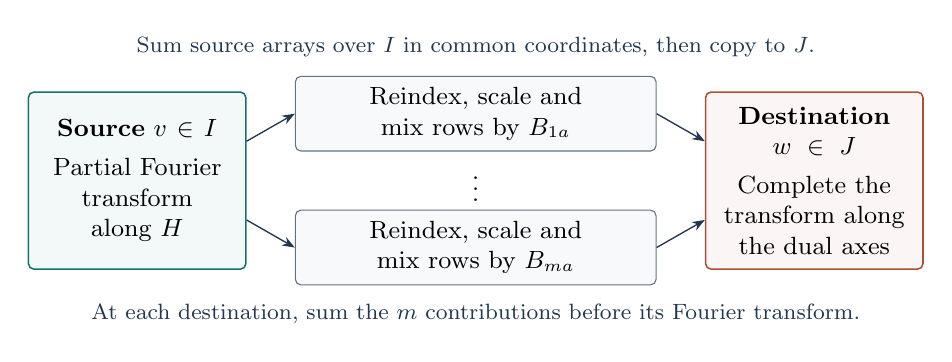
\begin{tikzpicture}[
  x=1cm,y=1cm,font=\small,align=center,
  endpoint/.style={draw=#1,fill=#1!5,line width=.55pt,rounded corners=2pt,
        text width=2.55cm,minimum height=2.25cm,inner xsep=3pt},
  query/.style={draw=ink!70,fill=ink!3,rounded corners=2pt,
        text width=4.3cm,inner sep=4pt},
  edge/.style={draw=ink,-{Stealth[length=1.6mm]},line width=.48pt}]
\node[endpoint=sea] (source) at (-4.3,0)
  {\textbf{Source \(v\in I\)}\\[3pt] Partial Fourier transform along \(H\)};
\node[endpoint=rust] (dest) at (4.3,0)
  {\textbf{Destination \(w\in J\)}\\[3pt] Complete the transform along the dual axes};
\node[query] (first) at (0,.85)
  {Reindex, scale and mix rows by \(B_{1a}\)};
\node[font=\small] at (0,0) {\(\vdots\)};
\node[query] (last) at (0,-.85)
  {Reindex, scale and mix rows by \(B_{ma}\)};
\foreach \op/\off in {first/5mm,last/-5mm}{
  \draw[edge] ([yshift=\off]source.east)--(\op.west);
  \draw[edge] (\op.east)--([yshift=\off]dest.west);
}
\node[font=\footnotesize,text=ink] at (0,1.7)
  {Sum source arrays over \(I\) in common coordinates, then copy to \(J\).};
\node[font=\footnotesize,text=ink] at (0,-1.7)
  {At each destination, sum the \(m\) contributions before its Fourier transform.};
\end{tikzpicture}
\caption{Fourier calls for one free rectangle \(I\times J\) and one power
\(a\). A source takes its partial transform once for all \(m\) queries.
Between the endpoints the common coordinates are \((x_C,y_C,s_1,t'_1)\)
in each column. The transposed destination transform acts along
\(H^\perp\). Both endpoint transforms use only auxiliary axes.}
\label{fig:route}
\end{figure}


\subsection{The finite saving and recursion}

Each endpoint uses at most \(2D\) calls per row incident to the
rectangle and per \(a\). For charged rectangles there are
\(O_L(q^t)\) common transforms per \(j,a\) across all \(q^L\) labels.
The number of calls in a pencil divided by the total \(Rq^L\) row
count is therefore at most
\begin{equation}
 \label{eq:kernel-pencil-cost}
 C_{\ell,L}D\bigl((1+\log q)^L + m q^{-(L-t)}\bigr).
\end{equation}
One full-row spectral conversion uses \(2d\) calls, also for the
inverse by frequency negation and scalar normalization. The repair
conversions therefore contribute \(O_\ell(dm^{-3})\) calls per row.
Choose \(q\) to be a power of two within a factor two of
\(m^{1/(L-t)}\). Then \(m q^{-(L-t)}=O_L(1)\).
The dimension estimate gives
\(D=O_{\ell,L}(m^{(\ell-1)/(L-t)})\). Given
\(0<\eta<\min(1,\theta-1/2)\), choose \(L\) large enough to make
\((\ell-1)/(L-t)<\eta\). The factor \((1+\log q)^L\) is then
absorbed by the remaining power of \(m\), so
Equation~\eqref{eq:kernel-pencil-cost} is \(O_{\ell,L}(m^\eta)\)
and \(D=o(m)\). Over all stages, the call count per row is at most
\[
 O_{\ell,L}\bigl(\sqrt{m\log m}\,m^\eta+dm^{-3}\bigr)
       =o(A^\theta).
\]
Here \(A=2(m+D-1)\). We may now fix \(m\equiv 1\pmod\ell\) large
enough to obtain the required strict saving at one recursion level.

The coefficients of the finite repair may lie in a fixed finite
free extension of \(R_\ell\). Expand each row in a basis of the
extension. A pointwise multiplication becomes a fixed matrix over
\(R_\ell\). Every axis call acts separately on basis components.
The target transform has base coefficients and the program accepts
arbitrary extension-valued input. Hence each basis component carries
an independent array over \(R_\ell\) and receives its own transform.
Expanding the scalars multiplies both the call count and the number
of input arrays by the extension rank. If \(W\) is the expanded number of rows and
\(\sigma\) the expanded number of calls, we have proved
\begin{equation}
 \label{eq:kernel-template-saving}
                          \sigma/W < A^\theta .
\end{equation}
For every \(f\ge1\), a batch contains \(W\) input and \(W\) output
rows of \(\ell^{Af}\) entries each. Each call acts on a single work
row of \(\ell^{Af}\) entries, applying \(D_\ell^{\otimes f}\) along
one axis for all \(\ell^{(A-1)f}\) fibers. An arbitrary common set of
spectator coordinates multiplies all these volumes equally. Outside
calls there are a fixed number of work rows and of linear passes.

Fix \(r\) so large that
\(b=(\sigma/W)(1+W/\ell^r)<A^\theta\). For a single \(k\)-digit array
take \(f=\lfloor(k-r)/A\rfloor\) when positive. The \(k-Af\) inactive
digits provide independent rows for the finite template. Batch these
rows with padding at the last batch. Handle the bounded number
\(k-Af<r+A\) of remaining digit transforms directly. The total work
divided by \(\ell^k\) satisfies
\[
                         T(k)\le C+bT(f).
\]
Indeed, each call runs the single-array algorithm independently on
its fibers and covers one full work row. The padding factor satisfies
\(\lceil\ell^{k-Af}/W\rceil W/\ell^{k-Af}\le 1+W/\ell^r\).
For bounded \(k\) use direct transforms. The ratio
\(b(1+f)^\theta/(1+k)^\theta\) has limit \(b/A^\theta<1\), so
induction gives \(T(k)=O((1+k)^\theta)\).

For uniformity, store the \(f\) columns in positional layout.
All index changes in the common-coordinate and representative
conversions apply a fixed linear change to each column. Interchanging
axes and changing strides in packing fibers also have known positional
weights. Enumerate column prefixes, extending each partial address
and its image by the next digit tuple times these weights. There are
a constant number of extensions per prefix and \(O(\ell^{Af})\)
prefixes. Along the same enumeration accumulate the phase exponents
and the \(m\) query exponents modulo \(\ell\). The query exponents
specify the repair table. All fixed ring constants have fixed expressions in
\(\zeta,1/\ell\) with integer coefficients. Normalization powers
depending on \(f\) take \(O(1+\log f)\) ring operations. These
procedures give linear work in local volume plus polynomial setup
in the local exponent, absorbed in that volume. Packing and
unpacking each batch requires a constant number of such traversals.
Address words of \(O(k+1)\) bits suffice, since the total number of
gates and temporary addresses is polynomial in \(\ell^k\). This
proves Theorem~\ref{thm:kernel}.


\subsection{Bit layout and stability for the Walsh--Hadamard transform}
\label{sec:binary}

At radix two, each recursive call transforms selected bits of an
address and leaves the other bits available for independent inputs.
The tape multiplication algorithm in \cite{oaT} uses this layout.
The same template also computes the normalized Walsh--Hadamard
transform. Its normalization can be absorbed into the recursive
calls, giving a fixed coefficient set and a bound on the accumulation
of numerical error.

\begin{proposition}[Binary implementations]\label{prop:binary-template}
Fix \(\theta>1/2\) and the arity \(A\), batch size \(W\) and call count
\(\sigma\) of Equation~\eqref{eq:kernel-template-saving} at \(\ell=2\).
\begin{enumerate}
\item An unnormalized batch on \(Af\) bits uses, outside its recursive
calls, pointwise linear maps on a fixed number of row entries, row
rewirings, and invertible \(\mathbb F_2\)-linear reindexings of the
\(A\) bits within each column. Its coefficients are drawn from a fixed
finite list of dyadic rationals and from signed powers of two with
exponent of magnitude \(O(f+1)\). Each call transforms a single
\(f\)-bit axis independently at every setting of the other bits.

The \(A\) axes may occupy contiguous slots consisting of \(f\) blocks
of \(K\) bits each. For any fixed \(0\le\rho<K\), the template can use
just bit \(\rho\) of each block. All other bits retain their addresses.
\item For even \(k\), the normalized transform \(2^{-k/2}D_2^{\otimes k}\)
has a uniform dyadic linear circuit of size
\(O_\theta(2^k(1+k)^\theta)\) with coefficients in a fixed finite
list outside the recursive calls. There are constants \(B,C,c>0\)
depending only on the template with the following property. If each
gate value is multiplied by \(1+\delta_g\), where
\(\lvert\delta_g\rvert\le u\le c(1+k)^{-B}\), the perturbed and exact
maps differ in Euclidean operator norm by at most \(Cu(1+k)^B\).
\end{enumerate}
\end{proposition}

\begin{proof}
The coefficient ring \(R_2=\mathbb Z[1/2]\) makes the fixed row
operations dyadic after descent. Table lookups use sums modulo two
of fixed column functions, and the phases are signs. The remaining
coefficients are powers of two from the axis normalizations and
from recovering the unnormalized target from the product \(F\).

By binary elimination each column reindexing is a fixed sequence of
additions from one axis to another, with an exchange implemented by
three additions. If \(x\) and \(y\) are the source and destination
slots for one such addition, the update is
\begin{equation}\label{eq:reindex}
 y_{\rho+iK}\longleftarrow y_{\rho+iK}+x_{\rho+iK}
       \quad\text{in }\mathbb F_2,\qquad 0\le i<f .
\end{equation}
Only the selected bits change. Fixing \(s\) inactive bits divides
one array of \(Z\) entries into \(2^s\) independent streams of
\(Z/2^s\) entries each. Group these streams into batches of \(W\),
padding the last batch. The recursive calls process in total
\[
 \sigma\lceil2^s/W\rceil\, Z/2^s
       \ \le\ (\sigma/W)(1+W/2^s) Z
\]
entries. This bound continues to hold for every slot width and offset.

For the normalized transform, take \(f\) to be the largest even
integer at most \((k-r)/A\) whenever this yields a positive child
width. The remaining \(k-Af<r+2A\) bits have even width and can be
handled by normalized four-point butterflies, as can the bounded
base cases. The padding bound and the strict saving in the recurrence
still apply.

Use a normalized transform in each axis call. For a common kernel
the \(2D\) calls supply the entire factor
\((2^{-f/2})^{2D}=2^{-Df}\). For a free rectangle the two partial
transforms together use those same \(2D\) axes. In a full spectral
conversion the common normalization commutes through its row table
and cancels with that of the inverse. Finally, \(F\) is already the
normalized target up to phases and a permutation. Thus all scalars
outside the recursive calls and the bounded remainder belong to a
fixed finite dyadic list.

Give the concatenated work rows their Euclidean norm. Each pointwise
stage is a direct sum of fixed-size circuits with bounded coefficients,
so its exact operator norm is bounded and perturbing its gates changes
the stage by \(O(u)\) for \(u\le1\). Permutations, zero padding and
restriction have norm at most one. Each recursive stage acts on
independent fibers by unitary transforms. Its perturbation has norm
bounded by the largest error on a fiber, even if different gates have
different errors. The number of successive stages per recursion level
is fixed. Telescoping their product therefore bounds the worst error
\(e(k)\) by \(C_0(u+e(f))\) whenever \(e(f)\le1\), with a constant
that includes the bounded remainder and base cases. The recursion
has depth \(O(1+\log_A(1+k))\). Iteration gives
\(e(k)\le Cu(1+k)^B\), and choosing \(c\) sufficiently small ensures
the child bound \(e(f)\le1\) at every level.
\end{proof}

Over \(\mathbb Q(\sqrt2)\) one can normalize odd widths as well.
Remove one bit from an odd-width call, apply \(2^{-1/2}D_2\) to that
bit, and use the even-width circuit on the rest. One may equally
normalize every axis call in a one-level template with arbitrary \(f\),
since its \(2D\) factors still multiply to \(2^{-Df}\). This retains
the call count, the inactive coordinates and the columnwise
reindexings. The scalars outside the calls now form a fixed finite
algebraic list. They can be approximated to \(p\) binary places in
time polynomial in \(p\) using dyadic arithmetic and the positive
root of \(2x^2=1\).



\part{All lengths over arbitrary fields}\label{part:all}
\section{Synchronized operations on tensor products}\label{sec:lay}

A finite abelian group may have many cyclic factors of unrelated orders.
Applying a separate algorithm along each axis can charge for a full pass
through the data each time. We construct circuits that perform the same
kind of operation on many axes in one pass. This requires control of
both the coefficients and the workspace. A shear with entries in the
prime field acts separately on each base coordinate of an extension
scalar. A transform that restores its scratch registers can borrow them
from neighboring input arrays, even after those arrays have been
transformed. These two facts let us synchronize transforms over an
extension and charge their cost to the original data. They will be used
first for polynomial multiplication in Section~\ref{sec:pack} and then
for the Fourier upper bound in Section~\ref{sec:last}. For related
synchronization and generation arguments see
\cite[Sections~2--3]{FiniteFourier}.

\subsection{Shears and permutations}

Put \(U=\left(\begin{smallmatrix}1&1\\0&1\end{smallmatrix}\right)\).
It adds one coordinate to another. The iterated shear \(U^{\otimes j}\)
acts on \(2^j\) coordinates and gives the basic layer for combining
operations on different axes.

\begin{lemma}[Tensor powers of a shear]\label{lem:shear}
For each \(\beta>1/2\) and every \(j\ge0\), \(U^{\otimes j}\) has a
binary linear circuit of size \(O_\beta(2^j(1+j)^\beta)\) over every
field, with an implied constant independent of the field.
\end{lemma}

\begin{proof}
Work first over an algebraic closure of the prime field. Use radix
\(\ell=2\) except in characteristic two, where we use \(\ell=3\).
On four coordinates consider the group generated by invertible
monomial matrices (permutations and diagonal scalings) and the Fourier
matrix \(D_\ell\) on any \(\ell\) of the coordinates, fixing the rest.
This group is \(\mathrm{GL}_4\). To see this, consider the tangent
spaces at the identity of its conjugates of the diagonal subgroup.
They contain all diagonal directions. Given \(i\ne j\), choose a
Fourier block containing \(i,j\). Conjugating a diagonal matrix unit
in the block by its Fourier matrix gives a matrix with a nonzero
\(ij\)-entry, because all entries of the transform and its inverse are
nonzero. Further conjugation by \(\operatorname{diag}(x_1,\ldots,x_4)\)
multiplies the \(ij\)-entry by \(x_i/x_j\). The distinct off-diagonal
characters and the constant character are linearly independent over
the algebraic closure. Taking linear combinations of these conjugates therefore isolates
the matrix unit in each off-diagonal position.

Choose finitely many of these tori whose tangent spaces span the space of
\(4\times4\) matrices. The multiplication map from their product to
\(\mathrm{GL}_4\) has surjective differential at the identity tuple.
Its image contains a nonempty open subset. Any translate of this open
subset meets it by irreducibility, so the generated subgroup equals
\(\mathrm{GL}_4\). In particular \(U^{\otimes2}\) has a finite word
in the generators. Inverses are again words, since Fourier inversion
uses only a permutation and a diagonal scaling in addition to the
forward transform.

The word length and the degree of its coefficient field over the prime
field can be bounded uniformly. Choose one word in characteristic zero.
Its coefficients lie in a number field and satisfy the matrix identity
for \(U^{\otimes2}\). Outside finitely many rational primes we may
reduce all coefficients at a prime of that number field, preserving
the identity and all nonzero scalars that are inverted. The residue
degrees are bounded by the number-field degree. In each exceptional
characteristic use the construction above.

For \(j=2r\), take the \(r\)th tensor power of this word over the
compositum with the given base field. Each monomial letter remains
monomial. A Fourier letter acts as \(D_\ell\) on a block and as the
identity on its complement. Its tensor power is a direct sum of
blocks \(D_\ell^{\otimes k}\), \(0\le k\le r\), obtained by fixing
the positions and labels outside the Fourier block. Their dimensions
sum to \(4^r\). Theorem~\ref{thm:kernel} therefore bounds the whole
letter by \(O_\beta(4^r(1+r)^\beta)\) gates. Describing the bounded-degree
extension in a base-field basis simulates every gate at constant cost.
The output matrix has base-field entries. For odd \(j\) apply the
remaining \(U\) on pairs of coordinates. The identity handles \(j=0\).
\end{proof}

A \emph{word} will be a sequence of invertible layers over an extension
field \(E\). A monomial layer permutes and rescales coordinates. A
\emph{shear layer} partitions the coordinates into blocks and applies
\(U^{\otimes j}\) to each block of size \(2^j\), allowing a different
\(j\) for each block. Singleton blocks are fixed. Permutations may
arrange the coordinates into the required blocks.

Tensoring two monomial layers gives a monomial layer. Tensoring two
shear blocks gives \(U^{\otimes(j_1+j_2)}\), so tensoring shear layers
gives a shear layer up to coordinate permutations. To tensor words of
length at most \(D\), assign a monomial slot and a shear slot to each
step and put the identity into each unused slot. The synchronized word
has length \(O(D)\), regardless of how many words are tensored. The
same schedule works for disjoint calls. An inverse word also has length
\(O(D)\), since \(U^{-1}\) is diagonally conjugate to \(U\).

When \(E\) contains a primitive \(s\)th root for \(s=\ell^j\), radix
recursion gives \(F_s\) a word of length \(O(1+\log s)\) on its \(s\)
coordinates \cite{CooleyTukey}. Each stage consists of disjoint
\(\ell\)-coordinate Fourier operations, diagonal scalings and
permutations. Gaussian elimination expresses any invertible operation
of this fixed size by a bounded number of monomial matrices and
elementary shears. A nonzero scalar shear is diagonally conjugate to
a unit shear.

\subsection{Evaluation and interpolation on a geometric progression}

For \(q\in K^\times\), the matrix
\(V_a(q)=(q^{ij})_{0\le i,j<a}\) evaluates a polynomial in the
power basis at \(1,q,\ldots,q^{a-1}\). The Newton basis converts both
evaluation and interpolation into a bounded number of triangular
Toeplitz operations over \(K\).

\begin{lemma}[Geometric Newton factorization]\label{up:newton-lemma}
Let \(V=V_a(q)\) have distinct nodes over \(K\). There is a lower
triangular matrix \(L\), diagonally equivalent over \(K\) to an
invertible triangular Toeplitz matrix, such that with
\(\Delta=\operatorname{diag}(L_{ii})\),
\begin{equation}\label{up:newton}
                         V=L\Delta^{-1}L^{\mathsf T}.
\end{equation}
Thus \(V\) and \(V^{-1}\) are bounded products of invertible diagonals
and invertible triangular Toeplitz matrices.
\end{lemma}

\begin{proof}
The \(j\)th Newton polynomial is \(\prod_{s<j}(X-q^s)\), where
\(0\le s<j<a\). Collect its power-basis coefficients in column \(j\)
of a unit upper triangular matrix \(P\). Its values form column \(j\)
of \(L=VP\), and vanish above the diagonal. Write
\(H_i=\prod_{k=1}^i(1-q^k)\), with \(H_0=1\). Evaluating the product
gives
\[
       L_{ij}=(-1)^j q^{\binom j2}H_i/H_{i-j}
               \qquad (0\le j\le i<a).
\]
Distinctness of the nodes makes each \(H_i\) nonzero. The lower
triangular Toeplitz matrix with coefficients \(1/H_k\) is therefore
diagonally equivalent to \(L\).

Now \(V=(L\Delta^{-1})\Delta P^{-1}\) is a unit
lower--diagonal--unit upper decomposition. Transposing and using
uniqueness for the symmetric matrix \(V\) gives
\(P^{-1}=(L\Delta^{-1})^{\mathsf T}\), proving \eqref{up:newton}.
An invertible lower triangular Toeplitz matrix represents multiplication
by a unit in \(K[X]/(X^a)\), whose reciprocal represents the inverse.
Transposition gives the upper triangular case. For this Newton change
of basis see \cite[Section~5]{BostanSchost}, for Vandermonde
factorizations see \cite{orucPhillips2000,kuznetsov2018}, and for their
implementation in circuits see \cite{FiniteFourier,ExplicitFourier}.
\end{proof}

\subsection{Using and restoring occupied workspace}

An axis transform will need scratch registers even when every coordinate
already holds data. The condition \(T\oplus I\) requires a word to
send \((x,z)\) to \((Tx,z)\) for \emph{every} initial value of the
scratch array \(z\). The identity on \(z\) makes a neighboring fiber
available as temporary storage. For earlier uses of restoration see
\cite{bennett1973,BuhrmanCleveKouckyLoffSpeelman2014,ExplicitFourier}.

\begin{lemma}[One factor with occupied workspace]\label{up:toeplitz}
Suppose \(2a\le b\le6a\), \(E\) contains a primitive \(b\)th root \(u\),
and a word of length \(D\) acts as \(F_b\oplus I\) on at most \(Cb\)
registers, where \(F_b=V_b(u)\). Let \(T\) be an invertible triangular
Toeplitz matrix of side \(a\), a geometric evaluation matrix with
distinct nodes, or the inverse of such an evaluation matrix, over
\(E\). A word of length \(O(D+1)\) acts as \(T\oplus I\) on
\(O((C+1)a)\) registers.
\end{lemma}

\begin{proof}
First implement \((x,y)\mapsto(x,y+Ax)\) for an arbitrary Toeplitz
matrix \(A\) of side \(a\). Write \(A=RLJ\), where \(J\) pads to \(b\)
coordinates, \(R\) truncates to \(a\), and \(L\) is a circulant.
The \(2a-1\) Toeplitz diagonals occupy distinct residues modulo \(b\).
For \(L\), transform the source and destination by \(F_b\), add the
scaled source entries using the diagonal \(F_b L F_b^{-1}\), and undo
the two transforms. The additions take one layer of scalar shears,
implemented by diagonal conjugation and unit shears. For \(J\) and
\(R\) the corresponding additions use disjoint unit shears.

For any two composable maps \(A_1,A_2\), the updates
\[
 z\gets z+A_1x,\qquad y\gets y+A_2z,\qquad
 z\gets z-A_1x,\qquad y\gets y-A_2z
\]
restore \(z\) and add \(A_2A_1x\) to \(y\). The contributions from the
original value of \(z\) cancel. Applying this identity twice implements
the addition for \(RLJ\), with a bounded number of length-\(b\)
transforms and \(O((C+1)b)\) registers.

To replace \(x\) by \(Tx\), first take \(T\) lower triangular Toeplitz.
Its action is multiplication by a unit \(h\) in \(E[X]/(X^a)\).
After dividing out the main diagonal we have \(h(0)=1\). Solve
\(f(uX)=h(X)f(X)\pmod{X^a}\) with \(f(0)=1\). The coefficient \(f_i\)
is determined by the earlier coefficients since \(u^i-1\ne0\) for
\(1\le i<a\). Write \(S\) for multiplication by \(f\) and
\(D_u=\operatorname{diag}(1,u,\ldots,u^{a-1})\). The identity for \(f\)
expresses \(T\) as \(D_u S D_u^{-1}S^{-1}\).

The additions associated to \(S\) and \(S^{-1}\) are available since
both matrices are Toeplitz. On two arrays they realize
\[
 \begin{pmatrix}I&S\\0&I\end{pmatrix}
 \begin{pmatrix}I&0\\-S^{-1}&I\end{pmatrix}
 \begin{pmatrix}I&S\\0&I\end{pmatrix}
 \begin{pmatrix}0&-I\\I&0\end{pmatrix}
  = B,\qquad B=\operatorname{diag}(S,S^{-1}).
\]
The last factor is a signed interchange. In
\((D_u\oplus I)B(D_u^{-1}\oplus I)B^{-1}\) the second block returns to
its initial value and the first block undergoes \(T\). Restore the main
diagonal by scaling. Reversing coordinates handles upper triangular
factors. For geometric factors and their inverses, successively apply
the words for the factors of Lemma~\ref{up:newton-lemma} using the same
scratch registers.
\end{proof}

\subsection{Borrowing registers across fibers}

Tensoring words that use \(Ca_i\) registers on the \(i\)th axis would
allocate as many as \(C^r\prod_{i=1}^r a_i\) registers. Instead we
borrow storage inside blocks of a fixed number of axes. A fiber along
one axis consists of the entries with every other coordinate fixed.

\begin{lemma}[Synchronizing axis operations]\label{up:fibers}
For each \(i\), suppose \(T_i\) acts on \(a_i\ge2\) coordinates and
a word of length at most \(D\) acts as \(T_i\oplus I\) on at most
\(Ca_i\) registers. Put \(B=\prod_i a_i\). A word of length
\(O_C(D+1)\) acts as \((\bigotimes_i T_i)\oplus I\) on \(O_C(B)\)
registers.
\end{lemma}

\begin{proof}
Put \(m=\lceil C\rceil\) and \(k=1+\lceil\log_2 m\rceil\). With at
least \(k\) factors, form blocks of \(k\) to \(2k-1\) factors. Within
one block, an axis of length \(a\) has at least \(2^{k-1}\ge m\)
fibers. Partition them into sets of \(m\) to \(2m\) fibers. Apply the
axis word to one fiber in each set, drawing its scratch registers from
the other fibers of that set. When the operation ends all borrowed
entries are restored. It is therefore possible to process the next
fiber even when the scratch space contains an earlier fiber's output.

Process all sets in parallel and the \(O_C(1)\) fibers per set in
sequence. Repeat for the \(O_C(1)\) axes of the block. This gives a
word of length \(O_C(D+1)\) on exactly the coordinates of each block.
Synchronizing their tensor product gives the same length bound on the
\(B\) data coordinates. With fewer than \(k\) factors, simply transform
one axis at a time, drawing disjoint scratch arrays from \(O_C(B)\)
additional registers for the simultaneous fiber calls. Every call
restores its array.
\end{proof}

\section{Polynomial convolution over arbitrary fields}\label{sec:pack}

Multiplying two polynomials of degree less than $n$ amounts to
computing the convolution of their two coefficient lists. If the field
contains suitable roots of unity, one can evaluate both polynomials,
multiply their values pointwise and interpolate. We will obtain the same
logarithmic exponent over fields that may lack those roots.

\begin{theorem}[Formal polynomial multiplication]\label{thm:conv}
For every $\alpha>1/2$, a division-free circuit over $K$ computes the
$2n-1$ coefficients of the product of two length-$n$ polynomials in
$O_\alpha(n(1+\log n)^\alpha)$ binary additions, subtractions and
multiplications. The count includes multiplication by prescribed scalars
and the implied constant is uniform over all fields $K$.
\end{theorem}

Each scalar in a root extension of degree $e$ occupies $e$ base-field
coordinates. We use each coordinate to hold input coefficients or
their products. The computation is a convolution on $N$ cyclic
addresses, carrying $r$ extension scalars per address as the
coefficients of a truncated polynomial.
Its total dimension $erN$ is comparable to the original length $n$.
Multiplying at one address reduces to ordinary convolution over $K$
at a length $O(er)$ whose logarithm is much smaller than $\log n$.

The choice of $N$ supplies a grid of small prime axes. In positive
characteristic the extension contains the required roots on every axis.
In characteristic zero we adjoin roots of order $p-1$ on an axis of
prime length $p$. A change of basis and a polynomial deformation then
give a pointwise multiplication using these shorter transforms.
Cantor and Kaltofen gave a convolution algorithm over arbitrary
algebras using $O(n\log n\log\log n)$ operations
\cite{CantorKaltofen}. For smooth extension degrees and many-axis
transforms in polynomial arithmetic see
\cite{harveyhoevenfinite,harveyhoevenconditional}.

\subsection{Packing the product without wraparound}

Suppose $E=K(\xi)$ has degree $e$, and choose positive integers $r,N$
with $8n\le erN\le9n$. Write $J_h=E[z]/(z^h)$ for truncated
polynomials of length $h$ (jets). In $J_r[X]/(X^N-1)$ the monomials
$\xi^a z^b X^j$, $0\le a<e$, $0\le b<r$, $0\le j<N$, form a
$K$-basis. To pack the inputs, reserve half of the room on each axis
for the growth in exponents when two monomials are multiplied.
Take radices
\[
 E_0=\lceil e/2\rceil,\qquad R=\lceil r/2\rceil,\qquad
 U=\lceil N/2\rceil.
\]
Since $E_0 RU\ge erN/8\ge n$, each input fits in the lower part of this
array. With $0\le a<E_0$, $0\le b<R$ and $0\le j<U$, place its coefficients
by the rule
\begin{equation}\label{poly:eq:mixed-radix-packing}
           a+E_0 b+E_0 Rj \quad\longmapsto\quad \xi^a z^b X^j,
\end{equation}
padding unused positions with zeros. The inequality
$2(\lceil k/2\rceil-1)<k$ applied at $k=e,r,N$ shows that
multiplying two occupied monomials adds their exponents without
reduction by the minimal polynomial of $\xi$, by $z^r$, or by $X^N-1$.

In the product, gather every coordinate $(a,b,j)$ with
$0\le a<e$, $0\le b<r$ and $0\le j<N$ by the integer $a+E_0 b+E_0 Rj$, retaining
indices $0,\ldots,2n-2$. Different triples can contribute to the same
index because of carries in the smaller radices. The index of each
product monomial is the sum of its two input indices, so gathering
gives ordinary convolution at all $2n-1$ outputs. Packing and
gathering cost $O(erN)$.

\subsection{Choosing the cyclic length and the field extension}

Put $T=\lceil\log n\rceil$. There is an absolute $C$ such that, with
$B=CT$ and for all sufficiently large $T$, there is a list of distinct odd primes
$p_i\le B$ whose product exceeds $n^2$ and
\[
 \log\mathrm{lcm}_i(p_i-1)=O(B^{4/5}\log B).
\]
We may omit any one forbidden prime. Shifted smooth primes have a similar role in matrix nonrigidity
\cite[Section~4]{DvirLiu}.
To see the claim, count primes $p\in[B/2,B]$
with $p\equiv1\bmod q$, summing over primes $B^{1/5}\le q\le B^{1/4}$.
By the Bombieri--Vinogradov theorem
\cite{BombieriV}, the sum is
\[
  (\operatorname{Li}(B)-\operatorname{Li}(B/2))
              \sum_q 1/(q-1)+O(B/(\log B)^2)
   = \Omega(B/\log B)
\]
by Mertens' theorem. Each $p$ is counted at most five times.
All prime factors of each $p-1$ are at most $B^{4/5}$, so
there are at most $B^{4/5}$ prime powers (largest power for each prime)
to include in the least common multiple, and each is at most $B$.
Taking $C$ large gives the claim.

Let $\ell=2$ except in characteristic two, where we take $\ell=3$.
This makes the radix invertible in $K$. In positive characteristic
also omit the characteristic from the list of primes.
In characteristic zero take primitive roots of all orders $p_i-1$,
and in positive characteristic take primitive roots of all orders $p_i$.
In both cases include a primitive root at the largest $\ell$-power
at most $8B$. Its powers supply the smaller radix lengths.
Let $E=K(\xi)$, where $\xi$ is a primitive root of order the least
common multiple of all these orders, and put $e=[E:K]$.

We claim that $\log e=O(B^{4/5}\log B)$. In characteristic zero
the order of $\xi$ bounds $e$, so the claim follows from the estimate
on the least common multiple of the $p_i-1$. In characteristic $b>0$,
we can choose $\xi\in\mathbb F_{b^D}$ for
\[
 D= \mathrm{lcm}_i(p_i-1)\cdot\varphi(\text{largest $\ell$-power up to $8B$}).
\]
Indeed $b$ is a unit modulo every required order. Its order modulo
$p_i$ divides $p_i-1$, and its order modulo any required $\ell$-power
divides the indicated totient. Hence $b^D-1$ is divisible by all the
orders. Since $E\subseteq K\mathbb F_{b^D}$, we have $e\le D$, as
required.

Take $N=\prod_{i=1}^d p_i$ from the longest prefix with
$eN\le n/B$.
Since $e=2^{o(T)}$ while the full product exceeds $n^2$, the
prefix is nonempty and has a next prime for all large $T$. That prime
is at most $B$ and would violate the upper bound, so
$n/B^2<eN\le n/B$. Choose an integer $r$ so that
\[
                8n\le erN\le 9n.
\]
The number $d$ of axes is at most $B$, and $B\le r\le9B^2$. In
particular
\[
             erN=\Theta(n),\qquad \log(6er)=O(T^{4/5}\log T).
\]
The first estimate accounts for the storage used by the packing above.
The second provides the saving in the recursive calls.

\subsection{Counting gates over the base field}

Let $M_K(j)$ denote the minimum circuit size of ordinary length-$j$
polynomial convolution over $K$. To charge a family of shorter
convolutions by its total operand length, put
$\mu_K(s)=1+\max_{1\le j\le s}M_K(j)/j$.

\begin{lemma}[Multiplication and shifts in jet coordinates]\label{poly:lem:descent-jet-cost}
Multiplication in $J_h$ costs $O(eh\mu_{K}(2eh))$ gates.
In characteristic zero, for any fixed $c\in K$, the shift $P(z)\mapsto P(z+c)$ of a
degree-$<h$ polynomial over $E$ costs $O(eh\mu_{K}(h))$ gates.
\end{lemma}
\begin{proof}
Represent the two jet inputs by bivariate polynomials of degrees $<e$
in $Y$ and $<h$ in $z$. Substitute $Y=w$ and $z=w^{2e-1}$. Raw product
exponents in $Y$ are at most $2e-2$, so the substitution separates the
rows of the product. Each packed operand has length at most $2eh$.
Multiply as ordinary polynomials over $K$. Keep the first $h$ rows and reduce each modulo the fixed monic minimal
polynomial $D$ of $\xi$ over $K$. For a row $V=DQ+S$ of degree $<2e$
with $\deg S<e$, reversing at degrees $2e-1,e,e-1$ gives
\begin{equation}\label{poly:eq:reciprocal-reduction}
  V^{\rm rev}\equiv D^{\rm rev}Q^{\rm rev}\pmod {Y^e}.
\end{equation}
Truncate $V^{\rm rev}$ modulo $Y^e$, multiply there by the precomputed
inverse of $D^{\rm rev}$, reverse the quotient, and subtract $DQ$. The two products per row
have operand lengths at most $e+1\le2e$. This reduction uses only
monicity and works over any coefficient ring. Together with the packed
product, all these multiplications have total operand length $O(eh)$.

For the shift, the new coefficient of $z^b$ is
\[
  \frac1{b!}\sum_{j=b}^{h-1} j!\,[z^j]P\,
                             \frac{c^{j-b}}{(j-b)!}.
\]
After reversal this is one fixed convolution of length $h$ per
$K$-coordinate, together with fixed scalings.
\end{proof}

A convolution with a fixed operand is a linear map at the same
asymptotic cost, even when the available multiplication circuit is an
arbitrary division-free circuit. Retain the constant and linear parts
of each wire in the remaining input. At a product gate the linear part
is $a_0b_1+a_1b_0$, where $a_0,b_0$ are precomputed constants.
The linear output is the required map.

Consider one layer of Section~\ref{sec:lay} on $V=O(N)$ registers
with entries in $J_h$. A shear block of size $2^j$ acts independently
on the $eh$ base-field coordinates of each entry. Since $j=O(1+T)$,
Lemma~\ref{lem:shear} bounds its cost by
$O_\beta(2^j eh(1+T)^\beta)$ for $\beta>1/2$. A monomial layer needs
at most $V$ multiplications by prescribed jet scalars. Summing the block sizes for the shear layer and applying
Lemma~\ref{poly:lem:descent-jet-cost} to the monomial layer bounds
the cost in either case by
\begin{equation}\label{poly:eq:descent-sync}
 O_\beta\big(Veh((1+T)^\beta+\mu_K(2eh))\big).
\end{equation}
For a tensor product of Fourier matrices of sides $a\le B$, suppose
their orders are invertible and their roots are in $E$. On each axis
take the least $\ell$-power at least $2a$, which is less than $6a$.
The roots for this auxiliary length are in $E$ by construction.
Radix stages and Lemma~\ref{up:toeplitz} give a word of
$O(1+\log B)$ layers on each axis with a bounded ratio of workspace
to data. Lemma~\ref{up:fibers} synchronizes the axis words in the same
depth and at constant total workspace overhead. Thus the cost of the
whole transform is Equation~\eqref{poly:eq:descent-sync} times
$O(1+\log B)$.

\paragraph{Positive characteristic.}
Chinese remaindering identifies the cyclic $N$-address space with a
$p_1\times\cdots\times p_d$ grid under componentwise addition.
Every axis order is invertible and $E$ contains a primitive root of
each order. Two forward transforms, $N$ products in $J_r$, and one
inverse transform therefore compute cyclic convolution. Fix
$1/2<\beta<\alpha$. Since $erN=\Theta(n)$, this costs at most
\begin{equation}\label{poly:eq:descent-cost}
 O_\beta\big(n(1+\log B)((1+T)^\beta+\mu_K(6er))\big).
\end{equation}
The argument in characteristic zero will allow jets of length $3r$,
which accounts for the factor $6$ here.

\subsection{A binomial coordinate on a prime axis in characteristic zero}

We now pass from the prime axis of length $p$ to an axis of length
$p-1$, whose roots lie in $E$.
Fix a prime $p$ from the list, put $m=p-1$, and choose a primitive
$m$th root $\omega\in E$. Let
$A=E[x]/(1+x+\cdots+x^{p-1})$.

\begin{lemma}[Prime cyclic algebra in binomial coordinates]\label{poly:lem:descent-prime}
There is a $\lambda\in E^\times$ and an isomorphism
\[
 E[x]/(x^p-1)\simeq E\times E[Y]/(Y^m-\lambda).
\]
The coordinate change in either direction has a word of
$O(1+\log p)$ layers on its $p$ coordinates with $O(p)$ restored workspace.
\end{lemma}
\begin{proof}
The factors $x-1$ and $1+x+\cdots+x^{p-1}$ are coprime since the
second takes the nonzero value $p$ at $1$. Chinese remaindering
gives a scalar coordinate by evaluation at $1$ and a second coordinate
in $A$. Choose a generator $g$ of $(\Z/p\Z)^\times$.
Order the nonzero residues by powers of $g$, as in Rader's
prime-length Fourier transform~\cite{rader}. The powers $x^{g^t}$ for
$0\le t<m$, with exponents taken modulo $p$, form a basis of $A$. They span since their sum is $-1$, and there
are $m=\dim_E A$ of them. The automorphism $x\mapsto x^g$ permutes
them cyclically. Its Fourier eigenbasis consists of the Lagrange resolvents
\[
 \gamma_j=\sum_{t=0}^{m-1}\omega^{-jt}x^{g^t},
 \qquad 0\le j<m,
\]
with eigenvalues $\omega^j$ and $\gamma_0=-1$. The algebra $A$ is
reduced because its defining polynomial has simple roots. Hence the
nonzero element $\gamma=\gamma_1$ has nonzero powers. In particular
$\gamma^m$ belongs to the invariant line $E\cdot1$ and equals a
nonzero scalar $\lambda\in E^\times$. Thus $\gamma$ is a unit even
when $A$ is a product of fields. For $1\le j<m$ we have
$\gamma^j=\kappa_j\gamma_j$ for some $\kappa_j\in E^\times$.
Thus $Y\mapsto\gamma$ identifies the binomial quotient with $A$.

In the cyclic algebra write an input as
$v_*+\sum_t v_t x^{g^t}$ and set $w_j=\sum_t\omega^{jt}v_t$.
Fourier inversion gives its image in $A$ as
$v_*+m^{-1}\sum_j w_j\gamma_j$. The coordinate in the scalar factor,
the constant coefficient in the binomial factor, and its positive-degree
coefficients are respectively
\[
  v_*+w_0,\qquad v_*-w_0/m,\qquad
  \frac{w_j}{m\kappa_j}\quad(1\le j<m).
\]
Lemma~\ref{up:toeplitz}, using the least $\ell$-power at least $2m$ as working length, applies the transform on its $m$
coordinates with restored workspace while leaving $v_*$ in place. The remaining two-coordinate
map has determinant $-p/m$, so it and its inverse have constant-length
words by elementary elimination and the shear construction.
The other steps are permutations and nonzero scalings.
The inverse transform is a forward transform at $\omega^{-1}$ followed
by scaling by $1/m$.
\end{proof}

For $p=3$ the nonconstant eigenvector is $\gamma=x-x^2$. The relation
$x^2+x+1=0$ gives $\gamma^2=-3$, so the binomial factor in this case
is $E[Y]/(Y^2+3)$.

The Chinese remainder isomorphism on the address group sends $X^j$
to the monomial of exponents $(j\bmod p_\nu)_\nu$. It identifies
$J_r[X]/(X^N-1)$ with the tensor product of the prime cyclic algebras
over $J_r$ by a permutation of coefficients. Apply
Lemma~\ref{poly:lem:descent-prime} on all axes and distribute this tensor
product over the scalar and binomial factors. The resulting blocks
are indexed by subsets $S\subseteq\{1,\ldots,d\}$. Writing
$m_\nu=p_\nu-1$, the block for $S$ is
\[
 \mathcal T_S=J_r[Y_\nu:\nu\in S]/
             (Y_\nu^{m_\nu}-\lambda_\nu:\nu\in S).
\]
Its width is $W_S=\prod_{\nu\in S}m_\nu$, and
$\sum_S W_S=\prod_\nu(1+m_\nu)=N$. By
\eqref{poly:eq:descent-sync} and Lemma~\ref{up:fibers}, both input conversions and the final inverse
conversion fit within \eqref{poly:eq:descent-cost}.

\subsection{Multiplying a block with one deformation parameter}
Fourier evaluation would multiply each block pointwise if its defining
binomials split, but $\lambda_\nu$ need not have an $m_\nu$th root in $E$.
We connect the block to one with relations $Y_\nu^{m_\nu}=1$ by varying a
single parameter $t$. We compute the product in a truncation at $t=0$
long enough to recover its coefficients as polynomials in $t$, then take
their Taylor expansions at $t=1$. Li, Moreno Maza and Schost used a common parameter
to deform relations in separate variables~\cite[Section~2.2, proof of Theorem~2]{triangularLMS}.
Bostan, Chowdhury, van der Hoeven and Schost developed the method for
triangular sets~\cite[Section~4.2, Proposition~7]{homotopyBCHS}.
Here the inputs themselves carry $r$ coefficients in the parameter,
and each binomial relation adds at most one to the degree required
for recovery.

\begin{lemma}[Multiplication through a split block]\label{poly:lem:descent-deform}
Let $H=2r+d$. Multiplication in $\mathcal T_S$ reduces to a tensor
Fourier transform on each of two arrays over $J_H$, one inverse tensor
transform, $W_S$ pointwise products in $J_H$, and a constant number
of jet scalings and polynomial shifts per basis monomial. The Fourier
axes have widths $m_\nu$, $\nu\in S$.
\end{lemma}
\begin{proof}
Use the $E[t]$-algebra
\[
 \mathcal A=E[t][Y_\nu:\nu\in S]/
 \bigl(Y_\nu^{m_\nu}-f_\nu(t):\nu\in S\bigr),
 \qquad f_\nu(t)=1+(\lambda_\nu-1)t.
\]
Its basis over $E[t]$ consists of the monomials whose exponent on each axis
is less than $m_\nu$, by successive division by the separate monic
relations. Use this same basis after each specialization. For the
$p=3$ example above the relation is $Y^2=1-4t$. In the product
$(a+bY)(c+dY)$ of two constant lifts, the scalar coefficient is
$ac+bd(1-4t)$. A single wrap changes its value from $ac+bd$ at $0$
to $ac-3bd$ at $1$.

Use $z_1=t-1$ for the parameter in $J_r$ at $t=1$, and $z_0=t$
for the parameter in $J_H$ at $t=0$. At the first endpoint, the map
from the specialized algebra to $\mathcal T_S$ sends the class of
$Y_\nu$ to $u_\nu Y_\nu$, where
$u_\nu^{m_\nu}=f_\nu(1+z_1)/\lambda_\nu$.
At the second endpoint the target is the split block with
$Y_\nu^{m_\nu}=1$. The corresponding map sends the class of $Y_\nu$
to $v_\nu Y_\nu$, where $v_\nu^{m_\nu}=f_\nu(z_0)$.
Each right-hand side has constant term one. The root with constant term
one exists and is unique, since the next unknown coefficient occurs
with multiplier $m_\nu\in E^\times$. These assignments respect the
defining relations and multiply each basis monomial by a unit.
We precompute that multiplier and its inverse for each monomial.

Start with two elements of $\mathcal T_S$ and undo the isomorphism
at $t=1$. For each coefficient choose its degree-$<r$ representative
in $z_1$ and substitute $t-1$ for $z_1$. These coefficients specify lifts
of the two elements to $\mathcal A$. In a product of basis monomials
$Y^aY^b$, the coefficient introduced by reduction is
\[
  \prod_{\nu\in S:\ a_\nu+b_\nu\ge m_\nu} f_\nu(t).
\]
Each axis contributes at most one factor, so the coefficient polynomials
of the lifted product have degree at most $2r-2+|S|<H$. Consequently their residues modulo $t^H$ give every coefficient of
the actual product polynomial. Reading these representatives in $E[t]$
lets us evaluate at $t=1+z_1$ even though the local calculation used
only jet arithmetic at zero (Figure~\ref{poly:fig:deformation}).
\begin{figure}[!htbp]
\centering
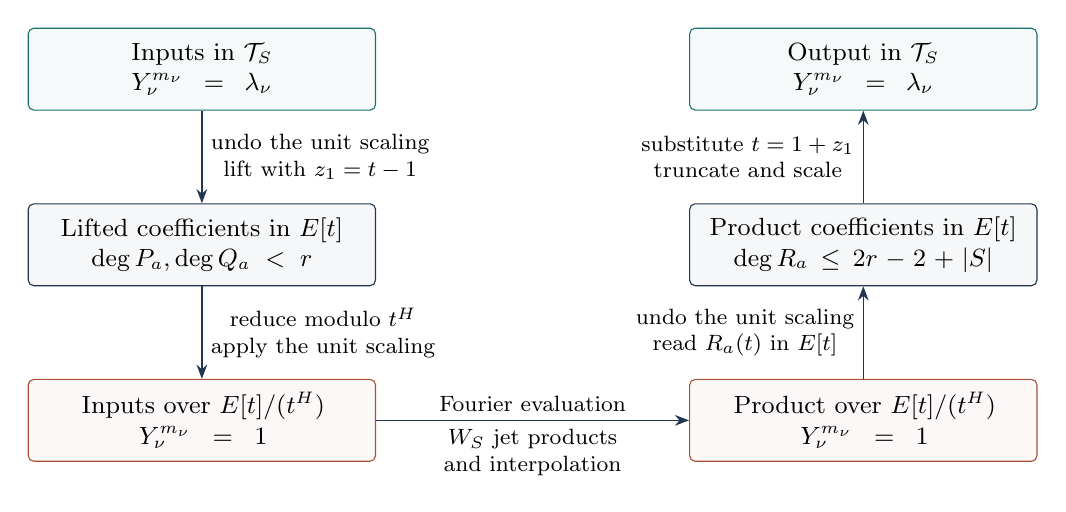
\begin{tikzpicture}[
  box/.style={font=\small,align=center,text width=4.2cm,minimum height=1.04cm,
              draw=#1,rounded corners=2pt,inner sep=3pt,fill=#1!4},
  labeltext/.style={font=\footnotesize,align=center,inner sep=3pt},
  arrow/.style={-{Stealth[length=1.8mm]},draw=ink,line width=.55pt}]
\node[box=sea] (in) at (0,0)
  {Inputs in $\mathcal T_S$\\$Y_\nu^{m_\nu}=\lambda_\nu$};
\node[box=sea] (out) at (8.4,0)
  {Output in $\mathcal T_S$\\$Y_\nu^{m_\nu}=\lambda_\nu$};
\node[box=ink] (lift) at (0,-2.23)
  {Lifted coefficients in $E[t]$\\$\deg P_a,\deg Q_a<r$};
\node[box=ink] (recover) at (8.4,-2.23)
  {Product coefficients in $E[t]$\\$\deg R_a\le2r-2+|S|$};
\node[box=rust] (splitin) at (0,-4.46)
  {Inputs over $E[t]/(t^H)$\\$Y_\nu^{m_\nu}=1$};
\node[box=rust] (splitout) at (8.4,-4.46)
  {Product over $E[t]/(t^H)$\\$Y_\nu^{m_\nu}=1$};
\draw[arrow] (in) -- node[labeltext,right] {undo the unit scaling\\lift with $z_1=t-1$} (lift);
\draw[arrow] (lift) -- node[labeltext,right] {reduce modulo $t^H$\\apply the unit scaling} (splitin);
\draw[arrow] (splitin) -- node[labeltext,above] {Fourier evaluation}
                        node[labeltext,below] {$W_S$ jet products\\and interpolation} (splitout);
\draw[arrow] (splitout) -- node[labeltext,left] {undo the unit scaling\\read $R_a(t)$ in $E[t]$} (recover);
\draw[arrow] (recover) -- node[labeltext,left] {substitute $t=1+z_1$\\truncate and scale} (out);
\end{tikzpicture}
\caption{Multiplication in a binomial block using one parameter for all
axes. The upper row uses length-$r$ jets at $t=1$ and the lower row
uses length-$H$ jets at $t=0$. Each axis wraps at most once in a
monomial product, so $H=2r+d$ captures every coefficient of the
ordinary polynomial in the middle row. This degree bound justifies
reading the polynomial before evaluating it at the other endpoint.}
\label{poly:fig:deformation}
\end{figure}


To compute these residues, pad the lifted coefficients to length $H$,
apply the isomorphism at zero, and evaluate at the $m_\nu$th roots of
unity on every axis. This identifies the split algebra with a product
of $W_S$ copies of $J_H$ because each Fourier evaluation is invertible
over $E$. Multiply pointwise, invert the tensor evaluation, and undo
the isomorphism at zero. Read the resulting length-$H$ coefficient
arrays as the actual product polynomials in $t$. Substitution of $1+z_1$
followed by truncation modulo $z_1^r$ specializes the product at the first
endpoint. The isomorphism there returns the required product in
$\mathcal T_S$. For $S=\varnothing$ the tensor evaluations are identities.
\end{proof}

For the three tensor transforms in a block $S$,
use \eqref{poly:eq:descent-sync} times $O(\log B)$, with volume
$V=W_S$, jet length $H\le3r$. The return transforms use
the same estimate as the forward transforms. The pointwise
products and the scales and shifts in the deformation lemma
also fit by Lemma~\ref{poly:lem:descent-jet-cost}
(shift by $\pm1$).
Summing over blocks proves the cyclic multiplication
bound~\eqref{poly:eq:descent-cost} in characteristic zero as well.

\begin{proof}[Proof of Theorem~\ref{thm:conv}]
Packing our ordinary convolution gives, in every characteristic and for all large $n$,
\[
 M_K(n)/n=O_\beta((1+\log T)((1+T)^\beta+\mu_K(6er))),
 \qquad \log(6er)=O(T^{4/5}\log T).
\]
For large $n$ we have $6er<n$. Induct on $n$ with the uniform
bound $M_K(n)/n\le C'(1+T)^\alpha$. The direct layer term contributes
$O_\beta((1+\log T)(1+T)^\beta)=o(T^\alpha)$.
Under the induction hypothesis the recursive term contributes at most
\[
  O_\beta\!\left((1+C')(1+\log T)
                       (1+T^{4/5}\log T)^\alpha\right)
     =(1+C')o(T^\alpha).
\]
Choose a threshold, independent of $K$ and $C'\ge1$, at which these
terms fit the claimed bound. Below it direct multiplication supplies
the base cases after increasing $C'$.
\end{proof}

\begin{corollary}[Fixed convolution and Toeplitz matrices]\label{cor:toe}
With $\alpha$ as above, any length-$n$ fixed convolution,
and hence any Toeplitz matrix on $n$ coordinates, has binary linear circuits over
the same field of size $O_\alpha(n(1+\log n)^\alpha)$.
\end{corollary}
\begin{proof}
Specialize one operand in Theorem~\ref{thm:conv} and retain the
linear parts at the gates. For a Toeplitz matrix $(t_{i-j})_{0\le i,j<n}$,
multiply the input polynomial by
$\sum_{k=-(n-1)}^{n-1}t_kX^{k+n-1}$ after padding to length $2n-1$.
The coefficient at $i+n-1$ is the desired output at $i$. These fixed
linear maps will supply the large axes in Section~\ref{sec:last}.
\end{proof}

\section{Geometric grids and the Fourier upper bound}\label{sec:last}

The character table of a finite abelian group factors into cyclic
character tables. The following result allows arbitrary geometric
progressions on the axes, allows interpolation in place of evaluation,
and admits triangular Toeplitz factors in the same product. Only the
prescribed factors must be defined over the base field. Auxiliary
Fourier transforms will take place in an extension whose coordinates
hold independent fibers of the original input.

\begin{theorem}[Geometric grids and triangular Toeplitz factors]\label{up:grid}\label{up:fourier}
Let \(K\) be any field, \(a_1,\ldots,a_r\ge2\), and \(N=\prod_i a_i\).
For each \(i\), let \(T_i\) be a matrix of side \(a_i\) over \(K\).
It may be the geometric evaluation matrix
\(V_{a_i}(q_i)=(q_i^{jk})_{0\le j,k<a_i}\) at distinct nodes with
\(q_i\in K^\times\), its inverse, or an invertible upper or lower
triangular Toeplitz matrix. For every \(\alpha>1/2\), the operator
\(\bigotimes_i T_i\) has a binary linear circuit over \(K\) of size
\(O_\alpha(N(1+\log N)^\alpha)\), with an implied constant uniform
in the field, the dimensions and the factors.
\end{theorem}

\begin{proof}
Fix \(1/2<\beta<\min(\alpha,1)\), put \(t=\lceil\log_2 N\rceil\) and
take \(c=1/24\). An axis of length \(a>N^c\) can be handled individually.
Corollary~\ref{cor:toe} applies a triangular Toeplitz factor on all
\(N/a\) fibers for \(O_\beta(N(1+t)^\beta)\) gates. By the Newton
factorization (Lemma~\ref{up:newton-lemma}), geometric evaluation and
its inverse satisfy the same bound. There are at most \(1/c\) such axes.

Group the smaller axes by multiplying their lengths until the product
first reaches \(N^c\), then start a new group. The last group may
fall short. There are \(O(1/c)\) groups and each has volume
\(B\le N^{2c}\). Fix one group. The \(h=N/B\) choices of complementary
coordinates supply \(h\) independent arrays, each of size \(B\).
Our two budgets for the group are a word of length \(O(1+\log t)\)
on \(O(B)\) registers, and an extension of degree at most \(h\).
The first will bound the number of passes through these arrays.
The second will let us fill the extension coordinates with data.

\paragraph{Choosing auxiliary lengths.}
A Fourier word for one factor of size \(a\le N^c\) needs a working
length \(b_a\) between \(2a\) and \(6a\) (Lemma~\ref{up:toeplitz}).
Directly padding to a power of the radix \(\ell\) could introduce
\(O(\log a)\) successive stages. We choose \(b_a\) with pairwise
coprime factors of size \(O(t^2)\). Their cyclic transforms can then
be synchronized and only the short factors need radix padding.

Use \(\ell=2\) except in characteristic two, where \(\ell=3\).
List the primes in \([t,t^2]\), omitting \(\ell\) and the
characteristic. By the prime number theorem their product exceeds
\(2N\) for large \(t\), even after the omissions. Let \(P\) be the
product of the longest prefix with \(P<2a\), taking \(P=1\) for the
empty prefix. Set \(b_a=P\ell^j\) for the least \(j\ge0\) with
\(P\ell^j\ge2a\). Then \(2a\le b_a<6a\). The next available prime
would have sufficed in place of \(\ell^j\), so \(\ell^j\le3t^2\).
The primes in \(P\) and this radix power give pairwise coprime
factors \(d\le3t^2\). For each \(d\ge2\), take the least power \(s_d\)
of \(\ell\) with \(s_d\ge2d\), so \(2d\le s_d<6d\).

Let \(M\) be the least common multiple of the lengths \(b_a,s_d\)
in this group and set \(E=K(\zeta_M)\) for a primitive \(M\)th root.
Every working length is prime to the characteristic and divides \(M\).
All the \(s_d\) are powers of one radix and their maximum is \(O(t^2)\).
If the group has \(k\) axes, then \(2^k\le B\), giving
\(\prod_a b_a\le6^k B\le B^4\), with one factor per axis. Hence
\begin{equation}\label{up:capacity}
               e=[E:K]\le M=O(t^2B^4)\le N/B=h
\end{equation}
for all sufficiently large \(N\), since \(B\le N^{1/12}\).

\paragraph{Constructing the word.}
Begin with the radix Fourier word of length \(O(1+\log t)\) on
\(s_d=O(t^2)\) coordinates from Section~\ref{sec:lay}.
Lemma~\ref{up:toeplitz} with \(a=d\), \(b=s_d\) gives a word of the same
order of length for \(F_d\), with \(O(d)\) registers.
Good's prime-factor factorization \cite{Good} expresses \(F_{b_a}\)
as the tensor product of these short transforms at appropriate primitive
roots, up to the Chinese remainder permutations on the input and output
indices. Lemma~\ref{up:fibers} synchronizes them within the same length
bound using \(O(b_a)\) registers.

Apply Lemma~\ref{up:toeplitz} a second time, now using \(F_{b_a}\) to
implement the prescribed factor \(T_i\) with \(a_i=a\). Synchronize these
axis words by Lemma~\ref{up:fibers}. The result is the desired word
of length \(O(1+\log t)\) on \(O(B)\) registers, acting as the tensor
product of the prescribed factors and restoring its other registers.
The original sizes \(a_i\) may be divisible by the characteristic.
Only the auxiliary Fourier lengths had to avoid it.

\paragraph{Returning to the base field.}\label{up:packing}
Let \(T\) be the transform of this group of axes. Pack \(e\) independent
input arrays \(x_0,\ldots,x_{e-1}\) entrywise in the power basis of
\(\zeta_M\). The intermediate word uses \(E\)-scalars, but \(T\) itself
has entries in \(K\). Thus each base coordinate returns its own answer,
\[
       T\left(\sum_{\nu=0}^{e-1}\zeta_M^\nu x_\nu\right)
        =\sum_{\nu=0}^{e-1}\zeta_M^\nu T x_\nu .
\]
By \eqref{up:capacity}, \(\lceil h/e\rceil\le2h/e\) batches suffice,
using zeros for unused coordinates of the last batch.

One monomial layer permutes or scales \(O(B)\) extension entries per
batch. Multiplication by a prescribed \(E\)-scalar costs
\(O_\beta(e(1+\log e)^\beta)\) binary linear gates over \(K\). Indeed,
multiply in the power basis and reduce modulo the fixed monic minimal
polynomial of \(\zeta_M\). The reversed quotient is a truncated product
of the reversed high coefficients with the reciprocal of the reversed
divisor. Subtracting the product of quotient and divisor gives the
remainder. Each convolution has one fixed operand, so
Corollary~\ref{cor:toe} supplies the stated bound. Over all batches
the layer costs \(O_\beta(N(1+t)^\beta)\), since \(e\le h\le N\).

A shear layer has blocks of total size \(O(B)\). On a block of size
\(2^j\) the entries of \(U^{\otimes j}\) lie in the prime field.
The block therefore acts independently on the \(e\) base coordinates.
By Lemma~\ref{lem:shear}, each costs \(O_\beta(2^j(1+j)^\beta)\)
gates. Since \(j=O(1+t)\), the entire shear layer also costs
\(O_\beta(N(1+t)^\beta)\) over all batches. There are \(O(1+\log t)\)
layers per group and boundedly many groups. The factor \(1+\log t\)
is \(O_{\alpha,\beta}((1+t)^{\alpha-\beta})\), which yields the claimed
bound. Direct circuits cover the finitely many smaller \(N\).
\end{proof}

\begin{proof}[Completion of the proof of Theorem~\ref{thm:main}]
Write a group as \(G=\prod_i C_{a_i}\), and choose a primitive
\(a_i\)th root \(q_i\) in the given splitting field. Its character
transform is \(\bigotimes_i V_{a_i}(q_i)\), up to the order of the
characters and group elements. Its inverse is the tensor product of the inverse factors. Theorem~\ref{up:grid} supplies a circuit
of size \(O_\alpha(N(1+\log N)^\alpha)\) for either choice. Applying
these circuits separately to the \(J\) independent blocks gives the
upper bound with one constant for all \(J\), all groups of the given
order and all common splitting fields. Together with the lower bound
this determines the exponent.
\end{proof}

\subsection{The logarithmic exponent of formal convolution}

Fixing one operand of a polynomial product makes the output linear in
the other operand. A suitable choice puts a cyclic Fourier transform
among the output coefficients. Extracting the linear part at every gate
then transfers the Fourier lower bound to division-free circuits for
multiplication.

\begin{corollary}[Independent formal convolutions]\label{cor:conv-exponent}
For every field \(K\), \(n\ge2\) and \(J\ge1\), let \(S_K(J,n)\) be
the minimum size of a binary division-free arithmetic circuit computing
\(J\) independent products of polynomials of degree less than \(n\).
All coefficients of all products are required as formal outputs. Then
there is an absolute \(c>0\) and, for each \(\alpha>1/2\), a constant
\(C_\alpha\) such that
\[
       cJn\sqrt{\log n}\ \le\ S_K(J,n)\
                  \le\ C_\alpha Jn(1+\log n)^\alpha .
\]
In particular the logarithmic exponent for formal convolution is
\(1/2\), uniformly in the field and the number of products.
\end{corollary}

\begin{proof}
Theorem~\ref{thm:conv} supplies the upper bound by computing each
product separately. For the lower bound, extend a size-\(s\) circuit
from \(K\) to \(\overline K\). For \(n\ge8\), choose
\(m=\lfloor n/2\rfloor\) or \(m=\lfloor n/2\rfloor-1\) invertible in
this field, and let \(q\) be a primitive \(m\)th root. Both lengths
are comparable to \(n\), and at most one is divisible by the
characteristic.

Bluestein's chirp identity \cite{Bluestein} uses the integer
\(b(k)=k(k-1)/2\), which satisfies \(b(i)+b(-j)-b(i-j)=ij\).
In each product set \(y_j=q^{b(-j)}x_j\) for \(0\le j<m\), using an
independent vector \(x\) for each block. Fix the other operand in every
block to the same polynomial \(H\), with coefficients
\(H_{m-1+d}=q^{-b(d)}\) for \(|d|<m\). Its \(2m-1\) coefficients fit
in length \(n\). Padding with zeros as needed gives, in each block,
\[
  q^{b(i)}[X^{m-1+i}]\left(H(X)\sum_{j=0}^{m-1} y_j X^j\right)
       =\sum_{j=0}^{m-1} q^{ij}x_j,\qquad 0\le i<m .
\]

Take the homogeneous linear part at each gate in \emph{all} remaining
variables together. Sums and differences combine the linear parts of
their arguments. At a product \(uv\) the linear part is
\(u(0)v_1+v(0)u_1\), using one binary linear gate for the linear
parts \(u_1,v_1\), even if both depend on many blocks. Input and output
scalings in the chirp identity can be absorbed into coefficients and
readouts. Thus a linear circuit with at most \(s\) gates computes
\(J\) independent Fourier transforms on \(C_m\). Theorem~\ref{thm:main}
gives \(s=\Omega(Jm\sqrt{\log m})=\Omega(Jn\sqrt{\log n})\).
For the finitely many smaller \(n\), the \(J(2n-1)\) output
coefficients are distinct nonzero quadratic forms. Each needs a gate
output distinct up to scalars from those for the others, which gives
the required linear bound in \(Jn\). The constants are uniform in
\(J\) and \(K\).
\end{proof}


\bibliographystyle{plainnat}
\bookmarksetup{startatroot}
\bibliography{references}
\end{document}
